\setcounter{chapter}{4}
\chapter{Teoria delle Perturbazioni}

Fino a questo a momento abbiamo visto che per risolvere l'equazione di Schr\"odinger per un determinato sistema, \`e sufficiente determinare gli autovalori associati all'operatore Hamiltoniano. In particolare nei capitoli precedenti si \`e dimostrato come nel caso dell'atomo d'idrogeno e dell'oscillatore armonico sia possibile ottenere delle soluzioni analitiche esatte. Nella realt\`a non sempre si riesce a definire una soluzione esplicita del problema, per questo motivo si \`e ricercato dei \textit{metodi di approssimazione} che ci permettano di ottenere delle soluzioni analitiche approssimate del sistema di partenza in alcuni casi.

Il primo caso che andiamo a discutere \`e in riferimento alla perturbazione di una Hamiltoniana non esplicitamente dipendente dal tempo.


\section{Teoria delle perturbazioni indipendenti dal tempo}

Supponiamo  di avere una sistema quantistico descritto da un operatore Hamiltonianano $\hat{H}_0$ indipendente dal tempo i cui autostati sono $|\phi_n \rangle $ e autovalori $E_{n}^0$, ovvero
\begin{equation*}
	\hat{H}_0 |\phi_m \rangle = E_m^0 | \phi_{m} \rangle \quad m \in \mathbb{N}
\end{equation*} 
Assumiamo che gli autostati $\vert \phi_n \rangle$ formi una base ortonormale completa dello spazio degli stati
\begin{equation*}
	\langle \phi_{k} | \phi_m \rangle = \delta_{km}
\end{equation*}
inoltre lo spettro associato all'operatore \`e discreto, e gli autovalori di $\hat{H}_0$ non hanno degenerazione.

La teoria delle perturbazioni \`e applicabile quando abbiamo un sistema descritto da una Hamiltoniana che pu\`o essere scritta come
\begin{equation}
	\hat{H} =  \hat{H}_0 + \lambda \hat{V}
\end{equation}
dove $\hat{V}$ \`e un operatore Hermitiano e $\lambda \in \mathbb{R}$. La Hamiltoniana $\hat{H}_0$ descrive la fisica del sistema imperturbato e il termine $\lambda \hat{V}$ prendere il nome di \textit{perturbazione}. La grandezza del parametro $\lambda$  definisce l'intensit\`a della perturbazione che si applica al sistema.

Se la perturbazione che applichiamo al sistema \`e indipendente dal tempo questa prende il nome di \textit{perturbazione stazionaria}. Inoltre afficnh\`e gli elementi di $\lambda \hat{V}$ siano molto pi\`u piccoli di quelli dell'operatore $\hat{H}_0$, imponiamo la condizione che il termine $\lambda \ll 1$.

Lo scopo del metodo delle perturbazioni \`e quello di espandere gli autovalori e autostati di $\hat{H}$ in potenze di $\lambda$, mantenendo un numero finito di termini. Assumiamo l'esistenza di un intorno $\Lambda$ del punto $\lambda = 0$ dove per ogni $\lambda \in \Lambda$, la Hamiltoniana perturbata $\hat{H}$ ha un singolo autovalore non degenere $E_n(\lambda)$ con autostato associato $|\psi_n(\lambda) \rangle $. Inoltre assumi che per $\lambda \in \Lambda$ si ha che 
\begin{align*}
	& \lim_{\lambda \to 0}E_n(\lambda) = E_n^0 \\[0.5cm]
	& \lim_{\lambda \to 0} |\psi_{n}(\lambda) \rangle = |\phi_n \rangle 
\end{align*}
Per definizione abbiamo che $E_{n}(\lambda)$ e $|\psi_n(\lambda)\rangle$ soddisfano l'equazione 
\begin{equation}
	\hat{H}|\psi_n \rangle = E_n |\psi_n \rangle 
\end{equation}
in cui assumiamo tacitamente la dipendenza da $\lambda$. Definiamo lo stato $|\psi_n \rangle$ come combinazione lineare degli autostati $|\phi_n \rangle$ dell'operatore imperturbato $\hat{H}_0$.
\begin{equation}
	|\psi_n \rangle = \sum_{m} C_{mn}|\phi_m \rangle 
\end{equation} 
dove i coefficienti $C_{mn}(\lambda) = \langle \phi_m| \psi_n (\lambda) \rangle $. Sostituendo (5.3) in (5.2) e usando l'espressione (5.1) otteniamo la espressione
\begin{equation*}
	\sum_{m} (E_n - E_m^0)C_{mn}|\phi_{m} \rangle = \lambda \sum_{m} C_{mn}V|\phi_m \rangle 
\end{equation*} 
Moltiplicando l'equazione precedente da sinistra per $\langle \phi_k |$ abbiamo che
\begin{equation}
	(E_n - E_k^0) C_{kn} = \lambda \sum_{m} C_{mn} \langle \phi_k|V|\phi_m \rangle  = \lambda \sum_{m}V_{km}C_{mn}
\end{equation} 
dove $V_{km} \equiv \langle \phi_k|V|\phi_m \rangle $. Vogliamo ora risolvere (5.4) rispetto ai coefficienti $C_{kn}(\lambda)$ e gli autovalori $E_{n}(\lambda)$. In particolare vogliamo trovare una soluzione perturbata rispetto ai termini di espansione $\lambda$. Dato che la funzione $| \psi_n(\lambda) \rangle $ \`e analitica per $\lambda \in \Lambda$, possiamo espandere i termine $C_{nm}(\lambda)$ come serie di potenze di $\lambda$:
\begin{equation}
\begin{array}{l}
C_{mn} ( \lambda)   = \langle \phi_m|\psi_n(\lambda) \rangle = \\[0.5cm]
 = \langle \phi_m | \Big( |\phi_n \rangle + \lambda |\psi_n^1 \rangle + \lambda^2|\psi_n ^2 \rangle + ... \Big ) = \\[0.5cm]
 = \delta_{nm} + \lambda \langle \phi_m|\psi_{n}^2 \rangle +  \lambda^2 \langle \phi_m| \psi_n^2 \rangle + ... = \\[0.5cm]
 \equiv \delta_{mn} + \lambda C_{mn}^1 + \lambda^2 C_{nm}^2 + ....   
\end{array}
\end{equation}
Dalla relazione (5.3) abbiamo che 
\begin{equation}
	|\psi_n ( \lambda) \rangle = |\phi_n \rangle + \lambda \sum_{m} C_{mn}^1|\phi_m \rangle + \lambda^2 \sum_{m} C_{mn}^2|\phi_m \rangle + ...
\end{equation}
Se $\lambda = 0$ l'equazione (5.4) si riduce alla condizione 
\begin{equation*}
	(E_n^0 - E_k^0)\delta_{kn} = 0
\end{equation*} 
Se $\lambda \neq 0$ e $\lambda \in \Lambda$, possiamo espandere gli autovalori $E_n(\lambda)$ in serie di potente di $\lambda$ nel seguente modo:
\begin{equation}
	E_n(\lambda) =\sum_{\alpha = 0}^{\infty} \lambda^\alpha E_{n}^{\alpha} = E_{n}^0 + \lambda E_n^1 + \lambda^2 E_n^2 + ... 
\end{equation}
Notare che per i termini $C_{nm}^\alpha$ e $E_n^\alpha$ gli esponenti sono solo nomenclature e non rappresentano delle potenze come nel caso di $\lambda$.

Sostituendo nell'equazione (5.4) per $\lambda = 0$  gli elementi (5.5) e (5.7) per poi raccogliere i termini con la stessa potenza in $\lambda$, otteniamo 
\begin{align}
	0  = & \delta_{kn} (E_n^0 - E_k^0) +  \notag \\[0.5cm] 
		& + \lambda \Big [ \delta_{kn}E_{n}^1 + C^1_{kn}(E^0_n-E_k^0) -V_{kn} \Big] + \notag \\[0.5cm]
		& + \lambda^2 \Big [ \delta_{kn}E^2_{n} + C^2_{kn}(E_n^0 - E_{k}^0) + C_{kn}^1E_n^1 - \sum_{m}V_{km}C_{mn}^1 \Big] + ...
\end{align}
di conseguenza tutti i coefficienti rispetto a $\lambda$ devono essere nulli. Il primo termine \`e automaticamente 0 per definizione. 

\subsection{Correzioni al primo ordine $\mathcal{O}(\lambda)$}

I coefficienti al primo ordine $\mathcal{O}(\lambda)$ sono nulli quando
\begin{align}
	& E_n^1 = V_{nn} \quad \quad \quad\quad k = n \\[0.5cm]
	& C_{kn}^1 = \frac{V_{kn}}{E^0_n - E^0_k} \quad \;k \neq n
\end{align}
Chiaramente notiamo che $C_{nn}^1$ non \`e determinabile dall'equazione (5.8).  Se moltiplichiamo l'equazione (5.1) ambo i lati per una costante Z arbitraria modifichiamo la norma di $|\psi_n \rangle$, ma non l'autovalore associato $E_n$
\begin{equation*}
	\hat{H}(Z|\psi_n \rangle) = E_n (Z|\psi_n \rangle)
\end{equation*}
questo ci dice che siamo libere di scegliere il valore di $\langle \psi_n | \psi_n \rangle $. Scegliamo di normalizzare $|\psi_n \rangle$ in modo tale che: 
\begin{equation}
	\langle \phi_n | \psi_n \rangle = 1
\end{equation}
Sostituendo (5.3) in (5.11) abbiamo che 
\begin{equation*}
	C_{nn}( \lambda) = 1
\end{equation*} 
e quindi usando la relazione (5.5) avremo la seguente equazione
\begin{equation}
	1 = C_{nn}(\lambda) = 1 + \lambda C_{nn}^1 + \lambda^2 C_{nn}^2 + ...
\end{equation}
di conseguenza affinch\`e l'identit\`a sia verificata dobbiamo avere che per i coefficienti per ogni potenza di $\lambda$ siano nulli  
\begin{equation}
	C^{\alpha}_{nn} = 0 \quad \alpha \in \mathbb{N}
\end{equation}
In conclusione possiamo riassumere i risultati ottenuti per le perturbazioni al primo ordine nel seguente modo:
\begin{align}
	& E_n( \lambda) = E_n^0 + \lambda \langle \phi_n | \hat{V} | \phi_n \rangle + ... \\[0.5cm]
	|\psi_n(\lambda) \rangle &= |\phi_n \rangle + \lambda \sum_{k \neq m} C_{kn}^1|\phi_k 
	\rangle + ... \notag \\[0.5cm]
	& = |\phi_n \rangle  + \lambda \sum_{k \neq n} \frac{\langle \phi_k|\hat{V}|\phi_n \rangle}{E_n^0-E_k^0}|\phi_k \rangle + ...
\end{align}
Queste due espressioni rendono chiaro il significato di "piccole perturbazioni". Dobbiamo avere che 
\begin{equation*}
	\langle \phi_n| \lambda \hat{V}|\phi_n \rangle \ll E_n^0
\end{equation*}
e
\begin{equation*}
	| \langle \phi_k| \lambda \hat{V} | \phi_n \rangle | \ll |E_n^0 - E_k^0|
\end{equation*}
Se le due condizioni non vengono rispettate, l'espansione ottenuta non \`e una buona approssimazione degli autovalori ed autostati della Hamiltoniana associata al sistema perturbato.

 L'espressione (5.15) ci dice che le correzioni al primo ordine degli autostati sono una serie infinita che dipende dagli elementi matriciali della perturbazione $\hat{V}$.
 
\subsection{ Correzioni al secondo ordine $\mathcal{O}(\lambda^2)$}

Consideriamo i termini al secondo ordine in $\lambda$. Il fatto che i coefficienti in $\lambda^2$ siano nulli ci porta ade avere le seguenti relazioni
\begin{align}
	& E_n^2 = \sum_{m} V_{nm}C_{mn}^1 - C^1_{nn}E_n^1  \quad \quad \quad k = n\\[0.3cm]
	& C^2_{kn} = \frac{1}{E_n^0-E_k^0} \Big( \sum_{m} V_{km}C_{mn}^1 - C_{kn}^1E_n^1 \Big  ) 
	\quad \quad \quad  k \neq n
\end{align}  
Usando i risultati (5.9),(5.10) e (5.13) le espressioni precedenti possono essere riscritte nel seguente modo:
\newpage 
\begin{align}
	& E_n^2 = \sum_{m \neq n} \frac{|V_{nm}|^2}{E_n^0-E_m^0} \quad \quad \quad k = n \\[0.3cm]
	& C^2_{kn} = \frac{1}{E_n^0 - E_k^9} \left( \sum_{m \neq n} \frac{V_{km}V_{mn}}{E_n^0-E_m^0} - \frac{V_{kn}V_{nn}}{E_n^0-E_k^0} \right) \quad \quad \quad k \neq n
\end{align}
Per scrivere (5.21) abbiamo usato il risultato che $V_{mn} = (V_{nm})^*$ dato che $\hat{V}$ \`e per ipotesi \`e un operatore autoaggiunto.
Utilizzando i risultati ottenuti fino a questo punto possiamo riscrivere i termini di grado pi\`u basso come 
\begin{align}
E_n^1 & =\left\langle\phi_n\right| \hat{V}\left|\phi_n\right\rangle \\[0.3cm]
\left|\psi_n^1\right\rangle & =\sum_{k \neq n} \frac{\left\langle\phi_k\right| \hat{V}\left|\phi_n\right\rangle}{E_n^0-E_k^0}\left|\phi_k\right\rangle \\[0.3cm]
E_n^2 & =\sum_{k \neq n} \frac{\left|\langle\phi_n | \hat{V}| \phi_k\rangle \right|^ 2}{E_n^0-E_k^0}
\end{align}

\begin{wrapfigure}{r}{0.4\textwidth} % 'r' for right, 'l' for left
    \centering
    \includegraphics[width=0.37\textwidth]{energystate} % Replace with your image file
    \label{fig:example}
\end{wrapfigure}
Se un sistema di trova al livello fondamentale $E_0^0$ nell'equazione (5.22) si ha a denominatore una grandezza $(E_0^0-E_m^0) < 0$ dato che  l'energia $E_0^0$ \`e il minimo valore che il sistema pu\`o assumere. 
In generale dalle perturbazioni al secondo ordine il livello fondamentale viene sempre abbassato.

\begin{wrapfigure}{l}{0.4\textwidth} % 'r' for right, 'l' for left
    \centering
    \includegraphics[width=0.37\textwidth]{energystate1} % Replace with your image file
    \label{fig:example}
\end{wrapfigure}
Per uno stato generico n-simo, si ah che per $n > m$ la perturbazione innalza il livello energetico, mentre per $m > n$ lo abbassa. Se sono presenti grandi spazi energetici tra i vari livelli si ha un contributo perturbativo minore rispetto a quelli pi\`u ravvicinati.

\subsection{Il coefficiente $C_{nn}^1$}

Per determinare il coefficiente $C^{1}_{nn}$ nella precedente sezione abbiamo scelto una normalizzazione dello stato $|\psi_n \rangle$ affinch\`e valesse la condizione (5.11). Inoltre tacitamente si \`e assunto che i termini fossero dei numeri reali, in realt\`a quando calcoliamo i coefficienti l'espressione (5.12) dovrebbe considerare il fatto che gli addendi $C_{nn}^{1}$ possono essere numeri complessi
\begin{align}
	1 & = \langle \psi_n| \psi_n \rangle = (\langle \phi_n| + \lambda \langle \psi_n|^1 +...)(|\phi_n \rangle + \lambda |\psi_n \rangle^1 +...) = \notag \\& = 1 +\lambda \langle \psi_n|^1\phi_n \rangle + \lambda \langle \phi_n|\psi_n \rangle^1 +... )=1 + \lambda(C^{1*}_{nn} + C_{nn}^1)+...
\end{align} 
 di conseguenza
 \begin{equation}
  C_{nn}^{1*} + C_{nn}^1 = 0
 \end{equation}
che equivale al sistema di equazioni

\begin{equation}
	\left \{ \begin{array}{l}
		Re(C_{nn}^1) = 0 \\[0.3cm]
		C_{nn}^1 = i\theta \quad \theta \in \mathbb{R}
	\end{array} \right.
\end{equation}
Dunque riscrivendo l'espansione dello stato $|\psi_n \rangle$ rispetto ai risultati in (5.17) abbiamo che
\begin{align*}
	|\psi_n \rangle & = | \phi_n \rangle  + \lambda (C_{nn}^1 | \psi_n \rangle + \sum_{m \neq n}C_{nm}^1 |\phi_m \rangle +...)+... = \\[0.5cm]
	& =(1+ \lambda C_{nn}^1)|\phi_n \rangle + \lambda\sum_{m \neq n}C_{nm}^1 |\phi_m \rangle +...)+... =   
\end{align*}
il termine $1+ \lambda C_{nn}^1 = 1 + \lambda i \theta$ coincide con lo sviluppo di Taylor arrestato al primo ordine della funzione $e^{i\lambda \theta}$ e quindi l'espressione precedente diventa
\begin{equation*}
	= e^{i \lambda \theta} (|\phi_n \rangle  + \lambda \sum_{m \neq n}C_{nm}^1|\psi_m \rangle +.. ) + ...
\end{equation*}
quindi abbiamo dimostrato che $C_{nn}^1$ non \`e necessariamente un termine nullo, ma pu\`o coincidere con un numero complesso di modulo unitario, che introduce un termine di fase che in meccanica quantistica pu\`o essere considerato trascurabile.

\section{Teoria delle perturbazioni indipendenti dal tempo degeneri}

Il problema \`e il medesimo di quello trattato nella sezione precedente solo che in questo caso assumiamo che i livelli energetici ammettano degenerazione.
Da un punto di vista qualitativo se $E_n^0$ \`e un autovalore degenere ci aspettiamo che i livelli reali siano sovrapposti e che l'introduzione di una perturbazione li separi.

Assumiamo che lo stato $E_n^0$ associato al sistema imperturbato possieda una degenerazione di  grado $g$; questo vuol dire che esiste un insieme di dimensione $g$ di autostati associati allo stesso autovalore.
\begin{equation}
	 \{ |\phi_n \rangle, |\phi_{n^1} \rangle, ....,|\phi_{n^g} \rangle \} 
\end{equation}
tutti associati al medesimo autovalore $E^0_{D}$,
\begin{equation*}
	E_n^0 = E_{n^1}^0 = \ldots =E_{n^g}^0 \equiv E_{D}^0
\end{equation*}
In questo caso a priori non possiamo imporre la condizione che 
\begin{equation}
	\lim_{\lambda \to 0 } |\psi_n \rangle = |\phi_n \rangle 
\end{equation}
siccome non sappiamo a quali valori dell'insieme (5.26) la funzione di stato $|\psi_n \rangle $ va a coincidere al ridursi del coefficiente perturbativo. Potrebbe anche convergere ad una loro combinazione lineare 
\begin{equation}
|\varphi\rangle=\left\langle\phi_n \mid \varphi\right\rangle\left|\phi_n\right\rangle+\left\langle\phi_{n^{\prime}} \mid \varphi\right\rangle\left|\phi_{n^{\prime}}\right\rangle+\ldots+\left\langle\phi_{n^{\prime \prime \ldots \prime \prime}}\mid \varphi\right\rangle\left|\phi_{n^{\prime \prime\ldots \prime \prime}}\right\rangle
\end{equation}
al tendere $\lambda \to 0 $. 
Data questa ambiguit\`a possiamo anche definire l'equazione del sistema senza indici
\begin{equation*}
	\hat{H}(\lambda)|\psi(\lambda) \rangle = E(\lambda)|\psi(\lambda) \rangle
\end{equation*}
ed espandiamo lo stato $|\psi \rangle $ rispetto alla base $\{|\phi_k \rangle \}$ isolando esplicitamente i contributi dati dagli stati degeneri associati al medesimo autovalore $E_{D}^0$
\begin{equation}
	|\psi(\lambda) \rangle = \sum_{m \in D} C_{m}(\lambda)|\phi_m \rangle + \sum_{k \not \in D}C_k(\lambda)|\phi_k \rangle
\end{equation}
dove $D = \{1,\ldots,g \}$ fa riferimento agli indici che identificano gli autostati degeneri.
Imponiamo la condizione per cui 
\begin{equation}
\lim_{\lambda \to 0} \equiv |\psi^0 \rangle = |\varphi \rangle 	
\end{equation}
dove, per definizione
\begin{equation}
	|\varphi \rangle = \sum_{m \in D} \langle \phi_m | \varphi \rangle |\phi_m \rangle  \quad \text{e} \quad \langle \varphi \mid \varphi \rangle = 1
\end{equation}
Dell'espressione (5.31) esistono almeno $g$ combinazioni lineari indipendenti possibili. Posto $\lambda = 0$ e utilizzando il risultato (5.30) abbiamo che l'equazione (5.29) assume la forma 
\begin{align}
	|\psi^0 \rangle & = \sum_{m \in D}C_{m}^0|\phi_m \rangle + \sum_{k \not \in D}C_{k}^0|\phi_k \rangle = \notag \\[0.5cm]
	& =  \sum_{m \in D} \langle \phi_m | \varphi \rangle |\phi_{m} \rangle 
\end{align}
dove abbiamo definito $C_{m}^0 \equiv C_m(\lambda = 0)$. Tale risultato ci dice che 
\begin{equation*}
	C_{k}^0 = \left \{ \begin{array}{l}
		\langle \phi_k|\varphi \rangle \quad k \in D \\[0.3cm]
		0 \quad \quad \quad \; k \not \in D
	\end{array}\right.
\end{equation*}
Ora procediamo come nel caso non degenere. Innanzitutto abbiamo che 
\begin{equation}
	(E - E_k^0) C_k = \lambda \sum_{m} V_{km}C_{m}
\end{equation}
Espandendo in serie di potenze coefficienti ed energie abbiamo 
\begin{equation*}
	C_k(\lambda) = C_k^0 + \lambda C_{k}^2 + \lambda^2 C_{k}^2 + \ldots 
\end{equation*}
 e
 \begin{equation*}
 	E(\lambda) = E_{D}^0 + \lambda E^1 + \lambda^2 E^2 + \ldots 
 \end{equation*}
 Sostituendo le due equazioni in (5.33) e raccogliendo i termini associati alla stessa potenza, abbiamo che 
 \begin{align}
0 & =  C_k^0\left(E_D^0-E_k^0\right) \notag \\[0.5cm]
& +\lambda\left[C_k^0 E^1+C_k^1\left(E_D^0-E_k^0\right)-\sum_m V_{k m} C_m^0\right] \notag \\[0.5cm]
& +\lambda^2\left[C_k^0 E^2+C_k^2\left(E_D^0-E_k^0\right)+C_k^1 E^1-\sum_m V_{k m} C_m^1\right]+\ldots
\end{align}
I coefficienti per ogni potenza di $\lambda$ devono essere nulli. 

\subsection{Correzioni al primo ordine $\mathcal{O}(\lambda)$}
Al primo ordine abbiamo che i coefficienti sono nulli quando valgono le seguenti condizioni 
\begin{align}
	& \sum_{m \in D} V_{km} \langle \phi_m|\varphi \rangle = E^1 \langle \phi_k| \varphi \rangle \quad \quad \;\; k \in D \\[0.5cm]
	& C_k^1(E_D^0-E_k^0) = \sum_{m \in D} V_{km} \langle \phi_{m} | \varphi \rangle \quad  k \not \in D
\end{align}
Chiaramente, le grandezze $V_{km}$ con $k,m \in D$, possono essere interpretate come elementi di una matrice $g \times g$. La relazione (5.35) pu\`o essere vista come un equazione rispetto agli autovalori che determina i $g$ autovalori $\{ E_{a}^2 \} = \{ E_{1}^1,E_{2}^2,...,E_{g}^1\} $ e i corrispondenti $g$ autostati $\{|\varphi_a \rangle  \} = \{ |\varphi_1 \rangle, |\varphi_2 \rangle ,...,|\varphi_g \rangle \} $. L'equazione (5.35) implica che in presenza di una perturbazione del sistema, l'insieme dei $g$ autostati degeneri $|\phi_n \rangle , |\phi_{n'} \rangle, \ldots , |\phi_{n^{'' \ldots ''}} \rangle  $ con autovalori $E_{D}^0$, vengono trasformati rispetto al primo ordine in un nuovo insieme di autostati $|\varphi_{1} \rangle, \ldots | \varphi_{g} \rangle $ con autovalori $E_{D}^0 + \lambda E_{1}^1,E_{D}^0 + \lambda E_{2}^1, \ldots,E_{D}^0 + \lambda E_{g}^1$.
Assumendo che i nuovi autovalori sia non degeneri, possiamo dire che \textit{la perturbazione ha rimosso la degenerazione}.

\section{Effetto Stark - Atomo d'idrogeno in un campo elettrico costante}

In questa sezione studiamo l'effetto Stark nell'idrogeno come esempio di teoria delle perturbazioni per uno stato legato. L'effetto Stark riguarda il comportamento degli atomi in presenza di un campo elettrico costante. 

Le prime osservazioni della divisione delle linee spettrali di un atomo per via dell'interazione con un campo elettrico sono state fatte da Stark nel 1913, che gli valse il premio Nobel nel 1919.
\newpage

\subsection{Sistema imperturbato}

Abbiamo un sistema costituito da un nucleo attorno al quale orbita un solo elettrone, ignorando lo spin delle particele, vogliamo studiare lo stato fondamentale dell'atomo d'idrogeno.

L'atomo a singolo elettrone viene modellato usando la Hamiltoniana che esprime un sistema a forza centrale 
\begin{equation}
	\hat{H}_0 = \frac{p^2}{2m} + V_0(r)
\end{equation}
dove per l'idrogeno abbiamo che
\begin{equation*}
	V_0 (r) = - \frac{e^2}{r}
\end{equation*}
Prima di iniziare a descrivere il sistema perturbato, abbiamo bisogno di capire il comportamento di quello imperturbato, a partire dalle sue energie, autostati e degenerazioni. Nel modello elettrostatico, i livelli di energia del sistema imperturbato sono descritti dalla formula Bohr
\begin{equation*}
	E_n = - \frac{1}{2n^2}\frac{e^2}{a_0} = -\frac{E_0}{n^2} \quad n \in \mathbb{N}
\end{equation*}
dove il termine $a_0$ indica il raggio di Bohr ed $E_0 = 13,6 \; eV$ l'energia associata allo stato fondamentale. Per l'atomo d'idrogeno gli atuovalori hanno una degenerazione di $n^2$. Gli autostati associati sono dati da 
\begin{equation*}
	|nlm \rangle = \psi_{nlm}(\bold{x}) = R_{nl}Y_{lm}(\theta,\phi)
\end{equation*}
dove le funzioni $Y_{lm}(\theta, \phi)$ sono armoniche sferiche.

\subsection{Potenziale}
Scriviamo la forza esterna $\bold{F}$ dovuta al campo elettrico esterno ed assumiamo che abbia orientazione lungo l'asse $\hat{u}_{z}$,
\begin{equation*}
	\bold{F} = F \hat{u}_{z}
\end{equation*}
Di conseguenza il potenziale della perturbazione ha forma
\begin{equation*}
	V_1 = q \phi = - q\bold{F} \cdot \bold{x} = eFz
\end{equation*}
dove si \`e considerato $q = -e $. Il potenziale imperturbato $V_0$ dipende da $r$, mentre quello perturbato $V_1$ dipende da $z$, di conseguenza abbiamo che la perturbazione del sistema rompe la simmetria di rotazione $SO(3)$ presente nel sistema imperturbato.

\subsection{Effetto Stark nello stato fondamentale}

Iniziamo la trattazione nel caso del sistema perturbato partendo dallo stato fondamentale dell'atomo di idrogeno; in notazione chimica coincide con la configurazione $1s$ che corrisponde all'autostato $| 100\rangle $. Siccome allo stato fondamentale non \`e presente degenerazione la correzione di energia al prima ordine \`e data da 
\begin{equation*}
	E^1_{0} = \langle 100|V |100 \rangle = 0 
\end{equation*}
che risulta essere nulla poich\`e 
\begin{equation*}
	\langle 100| eEz | 100 \rangle = eE \langle 100|z|100 \rangle  = eE\frac{1}{4 \pi} \int_{-\infty}^{\infty}dz z = 0 
\end{equation*}
dato che $z$ \`e una funzione dispari. Quindi possiamo concludere che al primo ordine per lo stato fondamentale dell'idrogeno non \`e presente una perturbazione al primo ordine dell'energia e di conseguenza nessun effetto Stark.
Osserviamo per\`o che  esiste una perturbazione del secondo ordine dello stato fondamentale, determinando
\begin{equation*}
	E_p^{(2)} = \sum_{q \neq p} \frac{|\langle \phi_q|V|\phi_p \rangle |^2}{(E_p^0-E_q^0)} = \sum_{nlm \neq 100} \frac{\langle nlm | eEz|100 \rangle|^2}{E_0/n^2-E_0} < 0
\end{equation*}
e quindi il livello $1s$ dell'atomo d'idrogeno viene abbassato di un ordine $\mathcal{O}(E^2)$. Resta comunque valida l'osservazione che non esista nessun effetto Stark per l'atomo d'idrogeno al livello fondamentale dato che questo coinvolge solo le perturbazioni del primo ordine delle energie.
\subsection{Effetto Stark negli stati eccitati dell'idrogeno}

Gli stati eccitati dell'idrogeno per $n \geq 2$ hanno una degenerazione tra gli stati con opposta parti\`a, dato che $l = 0,...,n-1$ e la parti\`a \`e pari per $l$ parti e dispari per $l$ dispari.  In accordo con la teoria descritta in precedenza per le perturbazioni di secondo ordine, la variazione dei livelli di energia $E_n$ \`e data dagli autovalori della matrice $n^2 \times n^2$, indicizzata da $(lm)$ e $(l'm')$
\begin{equation*}
	\langle nlm| eFz|nl'm' \rangle 
\end{equation*}
La matrice che si ottiene \`e di grandi dimensioni, ma molti elementi risultano essere nulli per motivi di simmetria. Consideriamo come esempio il caso per $n = 2 $. Abbiamo quattro stati degeneri inclusi nei livelli $2s$ con autostati $|nlm \rangle = |200 \rangle $ e il livello $2p$ con autostati $|21m \rangle $ con $m = 0, \pm 1$. 

Otterremo una matrice di  dimensione $4 \times 4$ i cui elementi si calcolano usando la relazione  $\langle \phi_i|V|\phi_j \rangle $ con $\phi_i = \{ \underbrace{ |211 \rangle, |21-1\rangle ,|210 \rangle }_{2p}, \underbrace{|200 \rangle}_{2s} \}$. Complessivamente la matrice possiede 16 elementi, per evitare di calcolarli tutti possiamo riassumerli sinteticamente nel seguente modo
\begin{equation*}
	\langle 200|z|200 \rangle  \sim \int_{-\infty}^{+\infty}dz  \; z = 0
\end{equation*}
per parit\`a della funzione $z$. 
\begin{equation*}
	\langle 21m|z|21m'\rangle \sim \int_{- \infty} ^{+ \infty}d\bold{x} \; Y_{1m}^*zY_{1m'} = 0 \quad m' \neq 0
\end{equation*}
gli elementi sono nulli per parit\`a. Gli unici termini non nulli della matrice sono dati da 
\begin{equation*}
	\langle 21m|z|200 \rangle \sim \int_{\mathbb{R}^3} d\theta() \int_{0}^{2\pi} d\varphi e^{im \phi} \sim \delta_{m0}
\end{equation*}

per $m = 0$ e dunque $\langle 210 |z|200 \rangle  = \alpha \in \mathbb{R}$. Dato che $\alpha$ \`e un numero reale anche $\langle 200| z |210 \rangle = \alpha$ che \`e il complesso coniugato di $\langle 210|z|200\rangle  $. Quindi possiamo concludere che la matrice di correzione \`e data da 
\begin{equation*}
	W = eE\left [ \begin{array}{cccc}
		0 & 0 & 0 & 0 \\
		0 & 0 & 0 & 0 \\ 
		0 & 0 & 0 & \alpha \\ 
		0 & 0 & \alpha & 0 \\
	\end{array} \right]
\end{equation*}
Procedendo a diagonalizzare la matrice si determinano i rispettivi autovettori
\begin{equation*}
	\left [ \begin{array}{c}
		1 \\ 0 \\ 0 \\ 0
	\end{array}\right ]
	;\quad 
		\left [ \begin{array}{c}
		0 \\ 1 \\ 0 \\ 0
	\end{array}\right ]
	;\quad 
	\underbrace{\frac{1}{\sqrt{2}}	\left [ \begin{array}{c}
		0 \\ 0 \\ 1 \\ 1
	\end{array}\right ]
	;\quad \frac{1}{\sqrt{2}}
		\left [ \begin{array}{c}
		0 \\ 0 \\ 1 \\ -1
	\end{array}\right ]}_{\text{autovettori della matrice di Pauli}\; \sigma_1}
\end{equation*}
i cui autovalori associati sono dati da $\Delta E = 0,0,eE,-eE$ e quindi i livelli energetici si dividono nel seguente modo.
\vspace{0.5cm}
\begin{center}
\begin{tikzpicture}
    % Draw all levels
    \text{2p} \draw[level] (0,0) -- node[above] {$|200 \rangle $} (4,0);
    \node[level,right] at (-1,0){2s};
    \draw[level] (4,0) -- node[above] {} (5,-0.25);
    \draw[level] (5,-0.25) -- node[below] {$\frac{|210 \rangle - |200 \rangle }{\sqrt{2}}$} (8,-0.25);
    
    \draw[level] (0,1) -- node[above] {$|21-1 \rangle$} (4,1);
    \draw[level] (4,1) -- node[above] {} (8,1);
    
    \draw[level] (0,2) -- node[above] {$|211 \rangle$} (4,2);
    \draw[level] (4,2) -- node[above] {} (8,2);
    \node[level,right] at (-1,2) {2p  };
    
    \draw[level] (0,3) -- node[above] {$|210 \rangle $} (4,3);
    \draw[level] (4,3) -- node[above] {}(5,3.25);
    \draw[level] (5,3.25) --node[above] {$\frac{|210 \rangle + |200 \rangle }{\sqrt{2}}$} (8,3.25);  
\end{tikzpicture}
\end{center}
Abbiamo rispettivamente che due livelli si alzano e abbassano e altri due restano imperturbati.
Lo splitting dei livelli \`e lineare rispetto alla perturbazione al primo ordine $\mathcal{O}(E)$.

\section{Forze di Van der Waals per due atomi d'idrogeno}

La caratteristica delle forze esercitate tra due atomi neutri cambia in funzione della distanza R che separa i due atomi. Consideriamo per esempio due atomi di idrogeno, quando R \`e dell'ordine atomico, la funzione d'onda dei due elettroni si sovrappongo, facendo attrarre i due atomi creando una molecola di $H_2$. L'energia potenziale del sistema ha un punto di minimo per un certo valore $R_e$ della distanza R tra gli atomi. L'origine dell'attrazione tra i due atomi \`e dovuta al fatto che i due elettroni oscillano tra di essi. In sostanza la funzione d'onda che descrive gli elettroni non \`e pi\`u localizzata attorno ad uno solo dei nuclei; una conseguenza di questo stato \`e che l'energia di stato fondamentale risulta essere pi\`u basse dei singoli atomi disaccoppiati.

A grandi distanza il fenomeno cambia completamente. Gli elettroni non possono pi\`u spostarsi tra i due atomi, dato che l'ampiezza di probabilit\`a del processo diminuisce al diminuire della sovrapposizione delle funzioni d'onda. L'effetto principale \`e dato dall'interazione elettrostatica tra i momenti di dipolo elettrico dei due atomi. Questo da luogo ad un energia complessiva dovuta a forze attrattive e decresce come $1/R^6$.  Tali forze prendono il nome di \textit{forze di Van der Waals} e sono responsabili per i legami chimici.

\subsection{Hamilotniana delle interazione elettrostatiche}

\begin{wrapfigure}{r}{0.5\textwidth} % 'r' for right, 'l' for left
    \centering
    \includegraphics[width=0.48\textwidth]{waals} % Adjust width as needed
\end{wrapfigure}

Dato che i due atomi sono sono neutri, a grande distanza l'interazione Coulombiana risulta essere nulla, dato che due elementi a carica neutra non si attraggono o respingono. Essendo per\`o composti da  particelle di carica opposta questi possiedono un momento di dipolo elettrico non nullo
\begin{equation*}
	\bold{d}_{A} = e\bold{r}_{A} \quad \text{e} \quad \bold{d}_{B} = e\bold{r}_{B}
\end{equation*}
Un atomo che possiede un momento di dipolo genera un potenziale elettromagnetico rilevabile anche a grande distanza e quindi l'atomo A risente del campo magnetico di B e viceverso. Di conseguenza abbiamo un interazione elettrostatica tra i due dipoli:
\begin{equation*}
	\Delta \phi = \frac{\bold{d}_{A} \bold{d}_{B}}{R^3} - \frac{3(\bold{d}_{A} \cdot \bold{R})(\bold{d}_{B} \cdot \bold{R})}{R^5}
\end{equation*}
dove $|\bold{r}_{A}, \bold{r}_{B}| \ll R$. Da cui il potenziale d'interazione \`e 
\begin{equation}
	V = \frac{e^2}{R^3}[\bold{r}_{A} \cdot \bold{r}_{B} - 3 (\bold{r}_{A} \cdot \bold{n})(\bold{r}_{B} \cdot \bold{n})]
\end{equation}
con $\bold{n} = \bold{R}/\parallel \bold{R}\parallel $. Se ipotizziamo che $\bold{R}$  parallelo alla direzione $\hat{u}_{z} $ possiamo scrivere (5.38) nella seguente forma
\begin{equation*}
	V = \frac{e^2}{R^3}[x_{A}x_{B} + y_{A}y_{B} -2z_{A}z_{B}]
\end{equation*}
La Hamiltoniana che descrive la dinamica del sistema \`e duque data da 
\begin{equation*}
	H_0 = - \frac{\hbar^2}{2m}(\nabla_{A}^2 + \nabla_{B}^2) - \frac{e^2}{r_{A}} - \frac{e^2}{r_{B}}
\end{equation*}
che descrive il sistema imperturbato e la somma del potenziale d'interazione V
\begin{equation*}
	H = H_0 + V
\end{equation*}
Lo stato fondamentale per il sistema imperturbato $H_0$ \`e dato dal prodotto tensoriale degli stati fondamentali dei corrispettivi atomi A e B, ovvero
\begin{equation*}
	|0 \rangle  = |100 \rangle_{A} \otimes |100 \rangle_{B}
\end{equation*}
\newpage 
\subsection{Correzioni al primo ordine $\mathcal{O}(E)$ per lo stato fondamentale}

Per determinare le correzioni al primo ordine calcoliamo
\begin{equation*}
	 \langle 0 | V | 0 \rangle  = 0
\end{equation*}
e risulta essere nulla, in quanto per come abbiamo definito il potenziale V, i termini $\langle 100|x_A|100 \rangle,\ldots, ecc \ldots$ hanno come armonica sferica $Y_{00} = 1/\sqrt{4 \pi }$ e dato che i fattori di V sono funzioni dispari si ha per parit\`a che tutti gli elementi sono nulli.

\subsection{Correzioni al secondo ordine $\mathcal{O}(E)$ per lo stato fondamentale}
Le correzioni al secondo ordine sono date da 
\begin{equation*}
	E^{(2)} = \frac{e^4}{R^6} \sum_{\substack{nlm  \\[0.1cm]  n'l'm'}} \frac{|\langle nlm|_{A}\otimes \langle n'l'm'|_{B})V(|100 \rangle_{A} \otimes |100 \rangle_{B})|^2}{2E_1 -E_n - E_{n'}}
\end{equation*}
abbiamo che in generale la sommatoria restituisce un termine negativo, e quindi un energia negativa di conseguenza si ha una forza di natura attrattiva. Possiamo dunque riassumere che le forze di Van der Waals hanno un ordine di grandezza rispetto alla distanza di $\simeq 1 / R^6$ e sono un effetto al secondo ordine della teoria delle perturbazioni.

\section{Struttura fine dell'atomo d'idrogeno}

\subsection{Ripasso sull'atomo d'idrogeno}

Sappiamo che la Hamiltoniana di un atomo d'idrogeno in un sistema imperturbato \`e data da
\begin{equation*}
	H_0 = \frac{\bold{p}^2}{2m} - \frac{e^2}{r}
\end{equation*} 
di cui conosciamo sia autostati e autovalori associati, ovvero $|nlm \rangle$ e $E_n = -E_0/n^2$. La Hamiltoniana $H_0$ che descrive l'interazione elettrone-protone \`e non relativistica, ovvero non consideriamo velocit\`a prossime a quella della luce e l'energia cinetica \`e quella data dalla meccanica Newtoniana.

Nella descrizione dell'atomo d'idrogeno del modello di Bohr la quantizzazione della velocit\`a cattura gli ordini di grandezza con cui si splittano i livelli di energia, infatti se consideriamo la velocit\`a al livello fondamentale abbiamo che 
\begin{equation*}
	v_1 = \frac{e^2}{\hbar } \equiv \frac{q^2}{4\pi \varepsilon \hbar}
\end{equation*}
se vogliamo considerare le correzioni relativistiche introduciamo la grandezza 
\begin{equation*}
	\frac{v_1}{c} = \frac{e^2}{c \hbar} \equiv \frac{q^2}{4 \pi \varepsilon c \hbar} \equiv \alpha = \frac{1}{137}
\end{equation*}
e prende il nome di \textit{costante di struttura fine}. Mentre l'energia allo stato fondamentale 
\begin{equation*}
	\frac{e^2}{a_0} = \frac{me^2}{\hbar^2} = \frac{m \alpha^2 \hbar^2 c^2}{\hbar^2} = \alpha^2 mc^2
\end{equation*}
Tali risultati ci dicono che la scala di energia dell'idrogeno \`e di un fattore $\alpha^2$ pi\`u piccola dell'energia a riposo dell'elettrone. Tenendo conto delle correzioni relativistiche possiamo riscrivere i livelli energetico come 
\begin{equation}
	E_n = - \frac{1}{2}\alpha^2 mc^2 \frac{1}{n^2}
\end{equation}
Il momento angolare associato all'idrogeno \`e 
\begin{equation*}
	p \simeq \frac{\hbar}{a_0} = \frac{me^2}{\hbar} = \frac{e^2}{\hbar c}mc \quad \rightarrow \quad p \simeq \alpha(mc)
\end{equation*}

La degenerazione dello spettro dell'atomo d'idrogeno \`e data dalla relazione
\begin{equation*}
	n = N+l+1
\end{equation*}
dove $N \geq $ \`e un polinomio di grado r che compare nella funzione d'onda dove la dipendenza di r in prossimit\`a dell'origine viene eliminata. Il numero quantistico $l \geq 0$ rappresenta il momento angolare dello stato. Per ogni $n$ fissato, il valore di $l$ \`e compreso tra zero e $n-1$. Per ogni valore fissato di $l$ l'autovalore di $L_z$ \`e $m \hbar$ con m che varia tra $-l$ ed $l$:
\begin{align*}
	& n = 1,2,... \quad \quad l = 0,1, \ldots, n-1 \\[0.5cm]
	& m = -l,\ldots,l \quad \quad \text{\# stati di energia } E_n = \sum_{l=0}^{n-1}(2l+1) = n^2
\end{align*}  
Gli stati dell'idrogeno possono essere riassunti nel seguente diagramma 
\begin{figure}[!ht]
\vspace{0.1in}
\includegraphics[width = 8cm]{hydrogen_states}	
\centering
\vspace{0.1in}
\end{figure}

Ogni autostato dell'atomo d'idrogeno \`e specificato dai tre numeri quantistici $n,l,m$ descritti dalle funzione d'onda
\begin{equation*}
	|nlm \rangle = A\left (\frac{r}{a_0}\right)^l \cdot \left ( \text{Polinomio in } \frac{r}{a_0}  \text{ di grado N}\right) \cdot e^{-r/na_0}Y_{l,m}(\theta ,\phi)
\end{equation*}
dove A \`e la costante di normalizzazione e $N = n - (l+1)$. Per lo stato fondamentale con $n=1,l=0$ e $m=0$ la funzione d'onda normalizzata \`e data da
\begin{equation*}
	|100 \rangle = \frac{1}{\sqrt{\pi a_0^3}}e^{-r/a_0}
\end{equation*}
Fino a questo punto nell'analisi di $H_0$ abbiamo ignorato lo spin dell'elettrone. Dato che un elettrone possiede spin $1/2$ \`e presente una degenerazione in pi\`u: ogni autostato di $H_0$ ha due stati di degenerazione, uno in cui si ha spin su e uno in cui si ha spin gi\`u. Questi stati sono degeneri perch\`e $H_0$ non ha termini dipendenza dallo spin.

Consideriamo due scelte differenti per la base degli stati dell'atomo d'idrogeno, entrambi che includono lo spin dell'elettrone.

Ricordiamo dalla trattazione dei momenti angolari accoppiati, che in generale per un momento $j$ accoppiato di due sistemi, abbiamo le coppie di stati $(j,m_j)$, dove $m_j$ varia da $-j$ a $j$ con incremento intero. Tutti gli stati composti sono autostati di $\bold{\hat{J}}^2$ con autovalori $\hbar^2j(j+1)$ e, per ogni stato, $\hbar m_j$ \`e l'autovalore di $\hat{J}_{z}$.

Dato che l'elettrone ha spin $1/2$ gli stati vengono indicati nel seguente modo
\begin{equation*}
	(s,m_s) \quad \text{con} \quad s=\frac{1}{2}, \quad m_{s} = \pm \frac{1}{2}
\end{equation*} 
Nell'atomo d'idrogeno il momento angolare $l$ pu\`o assumere diversi valori, ma lo spin dell'elettrone \`e sempre $1/2$. Per stati della base, questi sono descritti dai numeri quantici $n,l,m_l$ e $m_s$. Dato che non combiniamo lo spin dell'elettrone con il suo momento angolare, gli stati forma una base disaccoppiata
\begin{equation*}
	\mathcal{B} = \{|nlm_lm_s \rangle \} 
\end{equation*}
die elementi ortonormali tra loro.

Spesso \`e utile utilizzare una base alternativi dove gli stati sono autostati di $\hat{\bold{J}}^2$ e $\hat{J}_{z}$, dove il momento angolare totale $\bold{\hat{J}}$ \`e dato dalla somma del momento angolare orbitale $\bold{\hat{L}}$ e dallo spin della particella $\bold{\hat{S}}$:
\begin{equation*}
	\hat{\bold{J}} = \bold{\hat{L}} + \bold{\hat{S}}
\end{equation*}
Quando formiamo il prodotto tensoriale $l \otimes s$ stiamo considerando tutti i valori possibili di entrambi i numeri quantici. Tutti gli statti $l \otimes s$ sono autostati di $\hat{\bold{L}}^2$ e di $\bold{\hat{S}}^2$. Anche se gli stati non sono pi\`u autostati di $\hat{L}_{z}$ ed $\hat{S}_{z}$ lo sono ancora di $\hat{\bold{L}^2}$, quindi il numero quantistico $l$ sopravvive. La base accoppiata \`e descritta dai numeri quantici $(n,l,j,m_j)$.  I numeri $(m_l,m_s)$ della base disaccoppiata sono stati sostituiti da $(j,m_j)$. Gli stati accoppiati sono combinazione lineare di quelli disaccoppiati per cui si hanno differsi valori di $m_s$ e $m_l$, tali combinazioni restituisco lo stesso valore $m_j = m_l + m_s$.

Per determinare tutti gli stati accoppiati dobbiamo calcolare il prodotto tensoriale di ogni multicoppia $l$ dell'idrogeno con la coppia dello spin $1/2$. Le regole di addizione del momento angolare fanno si che il prodotto tensoriale assuma la forma
\begin{equation*}
	l \otimes \frac{1}{2} = \left (j=l + \frac{1}{2} \right ) \oplus \left (j = l-\frac{1}{2} \right )
\end{equation*}
PEr $l = 0$ otteniamo solo $j = 1/2$. Usando la notazione $L_j$ della tabella precedente con $L_j = S,P,D,F$ per $l = 0,1,2,3$. Il cambio della base \`e dato da 
\begin{equation*}
	l \otimes \frac{1}{2} \quad \rightarrow \quad L(l)_{j=l+ 1/2} \oplus L(l)_{j=l- 1/2}
\end{equation*}
o pi\`u esplicitamente
\begin{align*}
	& 0 \otimes 1/2 \quad \rightarrow \quad S_{1/2} \\[0.5cm]
	& 1 \otimes 1/2 \quad \rightarrow \quad P_{3/2} \oplus P_{1/2}\\[0.5cm]
	& 2 \otimes 1/2 \quad \rightarrow \quad D_{5/2} \oplus D_{3/2} \\[0.5cm]
	& 3 \otimes 1/2 \quad \rightarrow \quad F_{7/2} \oplus F_{5/2} 
\end{align*}
Usando questa notazione i multistati della base accoppiata, il diagramma dell'energia degli autostati dell'atomo d'idrogeno diventa 
\begin{figure}[!ht]
\vspace{0.1in}
\includegraphics[width = 8cm]{coupled_hydrogen_basis}	
\centering
\caption{Il numero di stati per ogni livello \`e segnato in parentesi}
\vspace{0.1in}
\end{figure}
\subsection{L'equazione di Pauli}

Nell'atomo d'idrogeno l'accoppiamento tra spin e momento orbitale nasce dal fatto che l'elettrone di muove nel campo elettrico del protone. Dato che l'elettrone si muove relativamente al riferimento dove si ha il campo elettrico, nel riferimento dell'elettrone questo risulta essere soggetto ad un campo magnetico $\bold{B}$. L'accoppiamento tra spin-momento \`e dovuto all'interazione tra momento di dipolo magnetico dell'elettrone $\boldsymbol{\mu}$ e il campo magnetico $\bold{B}$, dato da $- \boldsymbol{\mu} \cdot \bold{B}$. In unit\`a di Gauss, il momento magnetico per una spira in un piano attraversata da una corrente I \`e data da $\boldsymbol{\mu} = \frac{I}{c}\bold{a}$, dove $\bold{a}$ \`e il vettore dell'area racchiusa dalla spira. Pert una particella di carica q e massa $m$, questa possiede momento magnetico equivalente a quello della spira e dunque 
\begin{equation*}
	\boldsymbol{\mu} = \frac{q}{2mc} \bold{L}
\end{equation*}
dove $\bold{L}$ \`e il momento angolare orbitale dovuto alla rotazione. Per una particella elementare, lo spin della particella e il momento magnetico si associano similmente al momento angolare, ma con un fattore di proporzionalit\`a $g$
\begin{equation*}
	\boldsymbol{\mu} = g \frac{q}{2mc}\hat{\bold{S}}
\end{equation*} 
dove $g = 2$ per un elettrone. Dato che $q = -e$, abbiamo che il momento di dipolo \`e dato da 
\begin{equation*}
	\boldsymbol{\mu} = 2 \frac{-e}{2m_ec}\hat{\bold{S}} = -2 \frac{e \hbar}{2m_ec}\frac{\hat{\bold{S}}}{\hbar} = -2 \frac{e \hbar}{2m_ec} \frac{1}{2}\boldsymbol{\sigma} = - \frac{e \hbar }{2m_ec}\boldsymbol{\sigma}
\end{equation*}
In termine numerici il fattore di proporzionalit\`a \`e il \textit{magnetone di Bohr} $\mu_B$ definito come
\begin{equation*}
	\mu_{B} = \frac{e \hbar}{2m_ec} \simeq 9.274 \times 10^{-21} \frac{erg}{gauss} = 5.79 \times 10^{-9} \frac{eV}{gauss}
\end{equation*} 
(nel sistema internazionale 1 Teslata = $10^4$ gauss). L'effetto di accoppiamento tra elettrone e campo magnetico esterno \`e quindi descritto dalla Hamiltoniana $H_B$ data da
\begin{equation*}
	H_B = - \boldsymbol{\mu} \cdot \bold{B} = \frac{e\hbar}{2m_ec}\boldsymbol{\sigma} \cdot \bold{B}
\end{equation*}
Ora vogliamo dimostra che l'accoppiamento, e il valore $g=2$, compaiono naturalmente dall'equazione non relativistica di Pauli per un elettrone.

Consideriamo l'equazione indipendente dal tempo di Schr\"odinger per una particella libera
\begin{equation*}
	\frac{\bold{p}^2}{2m}|\psi \rangle = E|\psi \rangle
\end{equation*}
Dato che una particella con spin $1/2$ ha due gradi di libert\`a, l'equazione precedente pu\`o essere espressa in forma vettoriale come
\begin{equation*}
	\frac{\bold{p}^2}{2m} \mathbb{I}_{2 \times 2} \chi = E \chi \quad \text{con} \quad \chi = \left [\begin{array}{c}
		\chi_1 \\ \chi_2
	\end{array}\right]
\end{equation*}
dove $\chi$ viene anche chiamato \textit{spinore di Pauli}. Possiamo riscrivere la Hamiltoniana usando le matrici di Pauli ricordando l'identit\`a
\begin{equation*}
	(\boldsymbol{\sigma} \cdot \bold{a})(\boldsymbol{\sigma} \cdot \bold{b}) = \bold{a} \cdot \bold{b} \; \mathbb{I}_{2 \times 2} + i \boldsymbol{\sigma} \cdot (\bold{a} \times \bold{b})
\end{equation*}
considerando $\bold{a} = \bold{p} = \bold{\hat{p}}$, dove $\hat{\bold{p}}$ \`e l'operatore momento, e dato che $\hat{\boldsymbol{p}} \times \bold{\hat{p}} = 0$ abbiamo che la relazione precedente diventa
\begin{equation*}
	(\boldsymbol{\sigma} \cdot \hat{\boldsymbol{p}})(\boldsymbol{\sigma} \cdot \hat{\boldsymbol{p}}) = \bold{\hat{p}^2} \;\mathbb{I}_{2 \times 2}
\end{equation*}
di conseguenza possiamo riscrivere la Hamiltoniana nel seguente modo
\begin{equation}
	H = \frac{1}{2m} (\boldsymbol{\sigma} \cdot \hat{\boldsymbol{p}})(\boldsymbol{\sigma} \cdot \hat{\boldsymbol{p}})
\end{equation}
Fino a questo punto ci siamo solo occupati di scrivere la fisica in un altra forma, ma nuovi fenomeni emergono quando accoppiamo una particella carica ad un campo elettromagnetico esterno. In meccanica quantistica per tenere conto dell'accoppiamento sostituiamo la quanti\`a di moto canonica con 
\begin{equation*}
	 \hat{\bold{p}} \quad \rightarrow \quad \hat{\boldsymbol{\pi}} \;  \equiv \hat{\bold{p}} - \frac{q}{c} \bold{A}
\end{equation*}
dove q \`e la carica della particella ed $\bold{A}$ il potenziale vettore, che \`e una funzione della posizione che diventa un operatore dato che la posizione \`e un operatore. Inoltre, se \`e presente un potenziale elettromagnetico scalare $\Phi$ questo contribuisce alla Hamiltoniana con un termine aggiuntivo $q \Phi(\bold{\hat{x}})$. 

Sostituendo in (5.40) abbiamo che e con i termini aggiuntivi otteniamo quella che viene definita \textit{Hamiltoniana di Pauli}
\begin{equation}
	H_{Pauli} = \frac{1}{2m}(\boldsymbol{\sigma} \cdot \hat{\boldsymbol{\pi}})(\boldsymbol{\sigma} \cdot \hat{\boldsymbol{\pi}})+q \Phi(\hat{\mathbf{x}}) .
\end{equation}
utilizzando l'identit\`a delle matrici di Pauli usata in precedenza il termine di prodotto vettoriale sopravvive e possiamo esprimerla esplicitamente come
\begin{equation*}
H_{\text {Pauli }}=\frac{1}{2 m}[(\hat{\boldsymbol{\pi}} \cdot \hat{\boldsymbol{\pi}}) \mathbb{1}+i \boldsymbol{\sigma} \cdot(\hat{\boldsymbol{\pi}} \times \hat{\boldsymbol{\pi}})]+q \Phi(\hat{\mathbf{x}}) .
\end{equation*}
Abbiamo che $\boldsymbol{\hat{\pi}}\times \boldsymbol{\hat{\pi}} \neq 0$ perch\`e le singole componenti non commutano tra loro. Infatti
\begin{equation*}
	(\hat{\boldsymbol{\pi}} \times \hat{\boldsymbol{\pi}})_k=\epsilon_{i j k} \hat{\pi}_i \hat{\pi}_j=\frac{1}{2} \epsilon_{i j k}\left[\hat{\pi}_i, \hat{\pi}_j\right] .
\end{equation*}
dove il commutatore \`e dato da
\begin{equation*}
	\left[\pi_i, \pi_j\right]=\left[p_i-\frac{q}{c} A_i, p_j-\frac{q}{c} A_j\right] 
\end{equation*}
Le componenti dell'operatore $\bold{\hat{p}}$ possono essere viste come delle derivate agenti sulle corrispettive componenti spazialmente dipendenti di $\bold{A}$. Inoltre le componenti $A_i$, essendo funzioni della posizione, commutano tra di loro.
\begin{equation*}
	[\pi_i , \pi_j] = - \frac{\hbar}{i}\frac{q}{c}(\partial_i A_j - \partial_j A_i) = \frac{i \hbar q}{c}(\partial_i A_j - \partial_j A_i)
\end{equation*}
Possiamo scrivere esplicitamente le componenti del prodotto vettoriale sostituendo il risultato orrenuto 
\begin{equation*}
	(\boldsymbol{\pi} \times \boldsymbol{\pi})_k=\frac{1}{2} \epsilon_{i j k} \frac{i \hbar q}{c}\left(\partial_i A_j-\partial_j A_i\right)=\frac{i \hbar q}{c} \epsilon_{i j k} \partial_i A_j=\frac{i \hbar q}{c}(\nabla \times A)_k
\end{equation*}
riassumibile come 
\begin{equation*}
	\boldsymbol{\hat{\pi}} \times \boldsymbol{\hat{\pi}} = \frac{i \hbar q}{c} \bold{B}
\end{equation*}
In conclusione la Hamiltoniana di Pauli diventa
\begin{equation*}
	H_{Pauli} = \frac{1}{2m} \left( \bold{\hat{p}} + \frac{e}{c} \bold{A} \right)^2 + \frac{e \hbar }{2mc} \boldsymbol{\sigma} \cdot \bold{B} - e \Phi(\bold{\hat{x}})
\end{equation*}
Il secondo termine nella Hamiltoniana di Pauli espansa fornisce informazioni sull'accoppiamento tra lo spin dell'elettrone e il campo magnetico come discusso ad inizio sezione.

\subsection{L'equazione di Dirac }

Anche se l'equazione di Pauli incorpora nella sua espressione l'accoppiamento tra lo spin dell'elettrone e il campo magnetico, non \`e un equazione relativistica. Per poter includere la relativit\`a al suo interno, bisogna modificare le matrici e lo spinore di Pauli, portandole ad uno spinore a quattro componenti. Questo \`e dovuto al fatto che nella teoria relativistica si deve tenere conto delle antiparticelle.

Iniziamo con l'analizzare le relazioni tra le energie e le quantit\`a di moto relativistiche
\begin{equation*}
	E^2 - \bold{p}^2c^2 = m^2c^4 \quad \rightarrow \quad E = \sqrt{\bold{p}^2c^2 + m^2 c^4}
\end{equation*}
Tale relazioni ci suggerisce che un Hamiltoniana che tiene conto di fattori relativistici per una particella libera debba essere espressa come
\begin{equation*}
	H = \sqrt{\bold{\hat{p}}^2c^2 + m^2 c^4}
\end{equation*}
la cui equazione di Schr\"odinger associata \`e data da
\begin{equation*}
	i \hbar \frac{\partial \psi }{\partial t} = \sqrt{\bold{\hat{p}}^2c^2 + m^2c^4} \psi
\end{equation*}
Ipotizziamo che $p \ll mc$, e quindi espandiamo la Hamiltoniana utilizzando Taylor
\begin{align*}
	H & = mc^2 \sqrt{1 + \frac{\bold{\hat{p}}^2}{m^2c^2}} = mc^2 \left [1 + \frac{\bold{\hat{p}}^2}{2m^2c^2} - \frac{1}{8} \left ( \frac{\bold{\hat{p}}^2}{m^2c^2}\right)^2 + \ldots \right] = \\[0.5cm]
	& = mc^2 + \frac{\bold{\hat{p}}}{2m} - \frac{1}{8}\frac{\bold{\hat{p}}^4}{m^3c^2} + \ldots
\end{align*}
Se si ignora la massa costante a riposo, il primo termine coincide con quello della Hamiltoniana non relativistica e quello successivo \`e una correzione relativistica. Per piccoli valori della quantit\`a di moto possiamo considerare il termine correttivo come una perturbazione.

Dirac voleva determinare una Hamiltoniana lineare rispetto ai momenti e privi di radici quadrate. Questo \`e possibile se si scrivono le energie relativistiche come quadrato di una funzione lineare rispetto ai momenti:
\begin{equation}
	c^2 \bold{\hat{p}}^2 + m^2 c^4 = (c \boldsymbol{\alpha} \cdot \bold{\hat{p}} + \beta mc^2)^2 = (c \alpha_1 \hat{p}_1 + c \alpha_2 \hat{p}_2 + c \alpha_3 \hat{p}_3 + \beta mc^2)^2
\end{equation} 
\newpage
Espandendo i termine di destra ed uguagliando i coefficienti si trova che le seguenti relazioni sono verficate
\begin{align*}
	& \alpha_1^2 = \alpha_2^2 = \alpha_3^2 = \beta^2 = 1 \\[0.1cm]
	& \alpha_i\alpha_j + \alpha_j\alpha_i = \{ \alpha_i , \alpha_j \} = 0 \quad i \neq j  \\[0.1cm]
	& \alpha_i \beta + \beta \alpha_i = \{\alpha_i,\beta\} = 0
\end{align*}
Le relazione alla seconda e terza riga ci dicono che $\alpha$ e $\beta$ non possono essere numeri, perch\`e devono essere nulle. Di conseguenza si ha che $\alpha$ e $\beta$ sono matrici hermitiane $2 \times 2$
\begin{equation*}
	\boldsymbol{\alpha} = \left [ \begin{array}{cc}
		0 & \boldsymbol{\sigma} \\ \boldsymbol{\sigma} & 0
	\end{array} \right]  
	,\quad 
	\beta =  \left [ \begin{array}{cc}
		\mathbb{I} & 0 \\ 0 & -\mathbb{I}
	\end{array} \right]  
\end{equation*}
Usando la relazione (5.42) la Hamiltoniana di Dirac coincide con la funzione lineare del momento che \`e la radice quadrata di $c^2 \bold{\hat{p}}^2 + m^2 c^4$. Dunque abbiamo che
\begin{equation*}
	H_{Dirac} = c \boldsymbol{\alpha} \cdot \bold{p} + \beta m c^2
\end{equation*}
L'equazione di Dirac associata \`e 
\begin{equation*}
	i \hbar \frac{\partial \Psi}{\partial t} = (c \boldsymbol{\alpha} \cdot \bold{p} + \beta m c^2) \Psi
\end{equation*}
dove $\Psi$ \`e lo \textit{spinore di Dirac}, che corrisponde a un vettore colonna costituito da quattro componenti che pu\`o essere visto come composizione di due spinori di Pauli $\chi$ e $\eta$ a due componenti
\begin{equation*}
	\Psi = \left [ \begin{array}{c}
		\chi \\ \eta 
	\end{array}\right]
	,\quad
	\chi = \left [ \begin{array}{c}
		\chi_1 \\ \chi_2 
	\end{array}\right]
	 ,\quad
	 \eta = \left [ \begin{array}{c}
		\eta_1 \\ \eta_2 
	\end{array}\right]
\end{equation*}
L'accoppiamento al campo elettromagnetico viene tenuto conto considerando la trasformazione definita nella sezione precedente e quindi abbiamo che l'equazione di Schr\"odinger diventa
\begin{equation*}
	i \hbar \frac{\partial \Psi}{\partial t} = \left [ c \boldsymbol{\alpha} \cdot \left ( \bold{\hat{p}} + \frac{e}{c}\bold{A}\right) + \beta mc^2 + V(r) \right]\Psi
\end{equation*}
dove l'accoppiamento dell'elettrone viene introdotto considerando un potenziale scalare $\Phi(r)$
\begin{equation*}
	V(r) = - e \Psi(r) =- \frac{e^2}{r}
\end{equation*}
Il grande vantaggio dell'equazione di Dirac \`e che le correzioni della Hamiltoniana $H_0$ dell'idrogeno possono essere derivate in modo sistematica trovando l'appropriata Hamiltoniana H che agisce sullo spinore di Pauli $\chi$. L'analisi pu\`o essere fatta considerando $\bold{A} = 0$, dato che la stazionariet\`a del protone non genere vettore potenziale. Il risultato dell'analisi dimostra che 
\begin{equation*}
	H \chi = E \chi
\end{equation*} 
dove 
\begin{equation}
	H = \underbrace{ \frac{\hat{\bold{p}}^2}{2m} + V}_{H_0} - \underbrace{\frac{\bold{\hat{p}}^4}{8m^3c^2}}_{\delta H_{rel}} + \underbrace{\frac{1}{2m^2c^2r} \frac{1}{r} \frac{dV}{dr} \bold{S} \cdot \bold{L}}_{\delta H_{spin-orbita}} + \underbrace{\frac{\hbar^2}{8m^2c^2}\nabla^2 V}_{\delta H_{Darwin}}
\end{equation}
Il primo termine correttivo corrisponde a quello dell'energia relativistica come visto in precedenza. Il secondo termine rappresenta l'accoppiamento spin-orbita ed infine abbiamo la correzione di \textit{Darwin}, che come vedremo interagisce solo lo stato $l = 0$.

Ricordiamo che la scala energetica per gli autostati di $H_0$ \`e data da $\alpha^2 mc^2$. Vedremo che tutte le correzioni per alti livelli di energia sono dell'ordine di $\alpha^4 m c^2$ mentre di un fattore $\alpha^2$ le pi\`u piccole. Questo ci suggerisce che per l'atomo d'idrogeno , il ruolo del parametro $\lambda$ della teoria delle perturbazioni \`e dato dalla costante di struttura fine $\lambda \sim \alpha^2$.

Per le correzioni relativistiche, dove $p \simeq \alpha mc $, abbiamo che il primo termine diventa 
\begin{equation*}
	\delta H_{rel} = - \frac{\bold{p}^4}{8m^3 c^2} \sim - \alpha^4mc^2
\end{equation*}
Per la componente spin-orbita, riscriviamo il termine
\begin{equation*}
	\frac{1}{r}\frac{dV}{dr} = \frac{1}{r} \frac{d}{dr} \left( -\frac{e^2}{r}\right) = \frac{e^2}{r^3}
\end{equation*}
e quindi
\begin{equation*}
	\delta H_{spin-orbita} = \frac{e^2}{2m^2c^2} \frac{1}{r^3} \bold{S} \cdot \bold{L}
\end{equation*}
Stimiamo il proddotto spin e momento orbitale come $\bold{S} \cdot \bold{L} \sim \hbar^2 $, $r \sim a_0$, dove $a_0 = \hbar / mc \alpha$ e corrisponde al raggio di Bohr:
\begin{equation*}
	\delta H_{spin-orbita} \sim \frac{e^2}{m^2c^2} \frac{\hbar^2}{a_0^3} = \frac{\alpha \hbar c}{m^2 c^2}\frac{\hbar^2}{a_0^3} = \alpha \left( \frac{\hbar}{mca_0} \right )^3 mc^2 = \alpha^4 mc^2
\end{equation*}
Possiamo valutare il termine di Darwin ponendo $V = - e^2/r$:
\begin{equation*}
	\delta H_{Darwin} = - \frac{e^2 \hbar^2}{8 m^2 c^2} \nabla^2 \left( \frac{1}{r}\right) = \frac{e^2 \hbar^2}{8 m^2 c^2}(-4 \pi \delta(\bold{r})) = \frac{\pi}{2} \frac{e^2 \hbar^2}{m^2 c^2}\delta(\bold{r})
\end{equation*}
Per stimare questo termine correttivo notiamo che data la funzione $\delta $, l'integrale del valore di aspettazione introduce un fattore $|\psi(\bold{0})|^2 \sim a_0^{-3}$, e quindi abbiamo che
\begin{equation*}
	\delta H_{Darwin} \sim \frac{e^2 \hbar^2}{m^2 c^2 a_0^3} \sim \alpha^4 mc^2
\end{equation*}
che coincide esattamente con la stessa combinazione di costanti che otteniamo per il termine correttivo spin-orbita.

\subsection{Calcolo delle correzioni delle energie}

La struttura fine dell'atomo di idrogeno \`e lo spettro dell'atomo che tiene in considerazione i termini correttivi determinati fino ad ora. Date le semplificazioni viste nella sezione precedente 
\newpage
abbiamo che il sistema \`e descritto dalla Hamiltoniana 
\begin{equation}
	H=\underbrace{\frac{\hat{\mathbf{p}}^2}{2 m}+V}_{H^{(0)}}-\underbrace{\frac{\hat{\mathbf{p}}^4}{8 m^3 c^2}}_{\delta H_{\text {rel}}}+\underbrace{\frac{e^2}{2 m^2 c^2} \frac{\mathbf{S} \cdot \mathbf{L}}{r^3}}_{\delta H_{\text {spin-orbita }}}+\underbrace{\frac{\pi}{2} \frac{e^2 \hbar^2}{m^2 c^2} \delta(\mathbf{r})}_{\delta H_{\text {Darwin }}} .
\end{equation}
in questa sezione studieremo ciascuno dei singoli termini  e combineremo i risultati per determinare la struttura fine dell'atomo d'idrogeno.

Consideriamo i livelli energetici $|n\;l\;m\;s \;m_s \rangle $ dove $s = 1/2$ e $m_s = \pm 1$. Per l'atomo d'idrogeno sono presenti livelli di energia degeneri, senza spin la degenerazione \`e dell'ordine $n^2$, ma introducendolo abbiamo una degenerazione di $2n^2$ e quindi lo stato fondamentale \`e degenere due volte.

Calcoliamo i termini correttivi al primo ordine dell'energia determinando le componenti della matrice perturbativa $2n^2 \times 2n^2$ date da
\begin{equation*}
	\langle n' \; l' \; m' \; s \; m_s' \mid V \mid n \; l \; m \; s \; m_s \rangle 
\end{equation*}
diagonalizzandola otteniamo gli autovalori che correggono l'energia.

Per semplificare i conti possiamo scegliere una base particolare data dalle costanti del moto del sistema. La Hamiltoniana del sistema imperturbato $H_0$ \`e ha come costanti del moto 
\begin{equation*}
	[L,H] = [S,H] = 0
\end{equation*}
Dato che H in riferimento al sistema perturbato contiene il termine $\bold{L} \cdot \bold{S}$, abbiamo che $\bold{L}$ e $\bold{S}$ non sono pi\`u costanti del moto.  La costante del moto diventa il momento angolare totale del sistema $\bold{J} = \bold{L}+ \bold{S}$ poich\`e
\begin{align*}
	& [\bold{L}^2,H] = 0 \quad \rightarrow \quad [\bold{L}^2,L_i] = 0 \\[0.2cm]
	& [\bold{S}^2,H] = 0 \quad \rightarrow \quad [\bold{S}^2,S_i] = 0 \\[0.2cm]
	& [\bold{J}^2,H] = 0 \\[0.2cm]
	& [\bold{J}_i,H] = 0 \quad \rightarrow \quad [J_i,\bold{J}^2] = 0  
\end{align*}
Le prime due righe ci dicono che $\bold{L} \cdot \bold{S}$ commuta con $\bold{L}^2$ e $\bold{S}^2$. Dall'ultimo termine possiamo definire 
\begin{equation*}
	\bold{L} \cdot \bold{S} = \frac{(\bold{S} + \bold{L})^2- \bold{S}^2 - \bold{L}^2}{2} = \frac{\bold{J}^2 - \bold{S}^2-\bold{L}^2}{2}
\end{equation*}
Le costanti del moto sono dunque date da $\{\bold{J}^2,\bold{L}^2,\bold{S}^2,J_i,H\}$ e questo ci suggerisce di passare ad una base in cui consideriamo il momento angolare 
\begin{equation*}
	|n \; l \; s \; j \; m_j \rangle 
\end{equation*}
L'utilizzo di osservabili compatibili, fa s\`i che possano essere diagonalizzate simultaneamente e in modo equivaalente gli autostati della Hamiltoniana si organizzano in modo da essere autostati di ciascun osservabile.
Se prendiamo un certo livello $n$ a cui \`e associato un determinatore valore $l$, avremo che 
\begin{equation*}
	m = -l,\ldots,l \quad \text{e per} \quad s = \frac{1}{2} \rightarrow m_s = \pm \frac{1}{2} \quad \Rightarrow \quad |l-s| \leq j \leq l+s 
\end{equation*}
Complessivamente abbiamo $2(2l+1)$ stati di split del livello energetico.
\vspace{1cm}
\begin{center}
\begin{tikzpicture}
	\draw[level] (0,0) -- node[above]{l $m_l = -l, \ldots,l$} node[below]{s $m_s = -1/2,1/2$} (5,0);
	\draw[level] (5,0) -- node[above]{} (6,0.5);
	\draw[level] (6,0.5) -- node[above]{$j = l + 1/2 \quad m_j = -j,\ldots,j $} (13,0.5);
	\draw[level] (5,0) -- node[]{} (6,-0.5);
	\draw[level] (6,-0.5) -- node[below]{$j = l - 1/2 \quad m_j = -j, \ldots, j$} (13,-0.5);
\end{tikzpicture}
\end{center}
Lo spin si combina aumentando o diminuendo il momento angolare di $\pm 1/2$ e ogni livello si suddivide in due. In generale uno stato \`e dato da 
\begin{equation*}
	|nlsjm_j \rangle = R_{nl}(r) \{\text{momento angolare + spin}\}
\end{equation*}
dunque bisogna prendere le armoniche sferiche e gli stati con gli spin $\uparrow \downarrow$ e fare le opportune combinazioni lineari, gli elementi della matrice di perturbazione dipenderanno dalla componente radiale degli autostati.

Consideriamo il primo termine corretivo dato da $\delta H_{rel}$ il contributo al termine matriciale sar\`a dato da 
\begin{align*}
	\langle \ldots \mid - \frac{\bold{p}^4}{8m^3c^4}\mid \ldots \rangle & = \langle \ldots \mid -\frac{1}{2mc^2}\left( \frac{\bold{p}^2}{2m}\right)^2 \mid \ldots \rangle  = \\[0.3cm]
	& = \langle \ldots \mid - \frac{1}{2mc^2} \left ( E_n + \frac{e^2}{r}\right)^2 \mid \ldots \rangle = \\[0.3cm]
	& = \delta_{jj'}\delta_{m_jm_{j'}}\delta_{ll'} \left( \frac{4n}{l + 1/2} -3\right)\left( - \frac{E_n}{2mc^2}\right)
\end{align*}
Per il secondo termine correttivo $\delta H_{spin-orbita}$ dato dall'accoppiamento spin-orbita abbiamo che 
\begin{align*}
	\langle \ldots \mid \frac{1}{2m^2c^2}\frac{e^2}{r^3} \bold{L} \cdot \bold{S}|\ldots \rangle & = \langle \ldots \mid \frac{1}{2m^2c^2}\frac{e^2}{r^3} \frac{\bold{J}^2 - \bold{L}^2 - \bold{S}^2}{2} |\ldots \rangle = \\[0.4cm]
	& = \frac{\hbar^2}{2}[j(j+1)-l(l+1)-s(s+1)]\langle \ldots \mid \frac{1}{2m^2c^2}\frac{e^2}{r^3} \mid \ldots \rangle = \\[0.4cm]
	& = \frac{E_n^2}{mc^2} \frac{n(j(j+1)-l(l+1)-s(s+1)}{l(l+1)(l+1/2)}\delta_{jj'}\delta_{ll'}\delta_{m_j m_{j'}}
\end{align*}
Infine il terzo termine correttivo dato da $\delta H_{Darwin}$ ci restituisce un contributo all'elemento matriciale 
\begin{equation*}
	\langle \ldots | \frac{\hbar^2}{8 m^2 c^2}4 \pi e^2 \delta(\bold{r}) \mid \ldots \rangle = \frac{E_n^2}{mc^2}2n \delta_{jj'}\delta_{ll'}\delta_{m_j m_{j'}} \delta_{l0} 
\end{equation*}
dove il termine $\delta_{l0}$ \`e dovuto al fatto che si valuta la funzione in $\bold{r} = 0$, di conseguenza il contributo \`e non nullo solo per $l=0$ e quindi per $j = 1/2$.


Tutti i termini trovati sono diagonali rispetto alla base del momento angolare totale $\bold{J}$. Per l'atomo d'idrogeno i termini si combinano in modo tale che l'energia complessiva dipenda solo da $j$ e non da $l$. La formula per un livello di energia \`e 
\begin{equation}
	E_{nj} = - \frac{E_0}{n^2} \left[1 + \frac{\alpha^2}{n^2}\left(\frac{n}{j + 1/2} - \frac{3}{4} \right) \right]
\end{equation}
che corrisponde ad una correzione dell'ordine di $\alpha^2$ dei livelli energetici.

L'equazione di Dirac ammette soluzione esatta e la formula esatta degli autostati energetici \`e data da 
\begin{equation*}
	E_{nj} = mc^2 \left \{ \left [ 1 + \left( \frac{\alpha}{n-(j+1/2) + \sqrt{(j+1/2)^2-\alpha^2}}\right)^2\right]^{-1/2}-1 \right \}
\end{equation*}

\subsubsection{Esempio}
 Consideriamo il livello fondamentale per $n=1,l=0,j =1/2$ e $m_j = \pm 1/2$ si ha degenerazione, ovvero il livello energetico si splitta in due 
 \vspace{1cm}
\begin{center}
\begin{tikzpicture}
	\draw[level] (0,0) -- node[above]{$1S$}  (5,0);
	\draw[level] (5,0) -- node[above]{} (6,0.5);
	\draw[level] (6,0.5) -- node[above]{$j = 1/2  $} (13,0.5) node[right]{$1S_{1/2}$};
	\draw[level] (5,0) -- node[]{} (6,-0.5);
	\draw[level] (6,-0.5) -- node[below]{$j =  -1/2 $} (13,-0.5) node[right]{$1S_{-1/2}$};
\end{tikzpicture}
\end{center}
 Se consideriamo invece $n=2$ avremo due valori possibili del momento angolare $l = 0 ,1$ che in notazione spettroscopica sono i livelli $2S$ e $2P$. Per il livello 2s abbiamo che questo coincide con il livello $1S_{1/2}$, ottenendo una degenerazione in due livelli energetici. Per il caso $2P$ abbiamo una degenerazione di sei livelli energetici dato che per $l =1$ e $s = 1/2$ si ha $j = 1/2 , 3/2$, di conseguenza il livello 2P si spezza  in due a seconda del valore del momento 
 \vspace{1cm}
\begin{center}
\begin{tikzpicture}
	\draw[level] (0,0) -- node[above]{$2P$}  (5,0);
	\draw[level] (5,0) -- node[above]{} (6,0.5);
	\draw[level] (6,0.5) -- node[above]{$j = 3/2  $} (13,0.5) node[right]{$2P_{3/2}$};
	\draw[level] (5,0) -- node[]{} (6,-0.5);
	\draw[level] (6,-0.5) -- node[below]{$j =  1/2 $} (13,-0.5) node[right]{$2P_{1/2}$};
\end{tikzpicture}
\end{center} 
a loro volta il livello energetico $2P_{3/2}$ si divide in altri quattro livelli di energia dato che $m_j = -3/2,-1/2,1/2,3/2$, mentre $2P_{1/2}$ in altri due dato che $m_j = - 1/2,1/2$.

Che graficamente possiamo rappresentare come 
\newpage

\vspace{1cm}
\begin{center}
\begin{tikzpicture}
	\draw[level] (0,0) -- node[above]{$2P$}  (3,0);
	\draw[level] (3,0) -- node[above]{} (4,0.5);
	\draw[level] (4,0.5) -- node[above]{$2P_{3/2}$}(6,0.5) ;
	\draw[level] (6,0.5) -- node[right]{}(7.5,1.5);
	\draw[level] (7.5,1.5) -- (9.5,1.5)node[right]{$m_j = 3/2$};
	\draw[level] (6,0.5) -- (7.5,1);
	\draw[level] (7.5,1) -- (9.5,1) node[right]{$m_j = 1/2$};
	\draw[level] (6,0.5) -- node[right]{}(7.5,-0.5);
	\draw[level] (7.5,-0.5) -- (9.5,-0.5)node[right]{$m_j = -3/2$};
	\draw[level] (6,0.5) -- (7.5,-0.);
	\draw[level] (7.5,-0.) -- (9.5,0.) node[right]{$m_j = - 1/2 $};
	\draw[level] (3,0) -- node[]{} (4,-2);
	\draw[level] (4,-2) -- node[below]{$2P_{1/2}$} (6,-2) ;
	\draw[level] (6,-2) -- (8,-1.5);
	\draw[level] (8,-1.5) -- (9.5,-1.5) node[right]{$m_j = 1/2$};
	\draw[level] (6,-2) -- (8,-2.8);
	\draw[level] (8,-2.8) -- (9.5,-2.8) node[right]{$m_j = - 1/2$};
\end{tikzpicture}
\end{center} 
La struttura fine separa i livelli energetici dell'atomo d'idrogeno, ma li lascia degeneri. La degenerazione \`e dovuta al fatto che il numero quantico $m_j$ essendo la proiezione del momento angolare in una direzione, fino a quando non viene rotta la simmetria sferica del problema, questo viene conservato. 

Il modulo del momento pu\`o essere arbitrario, ma la proiezione nello spazio \`e rilevante e l'assenza di $m_j$ nell'equazione dell'energia \`e spiegata dall'invarianza per rotazioni del problema.

\section{Teoria delle perturbazioni dipendenti dal tempo }

Abbiamo discusso fin'ora della meccanica quantistica di sistema la cui Hamiltoniana \`e indipendente dal tempo, in questi casi la dipendenza temporale dei pacchetti d'onda pu\`o essere espressa mediante l'operatore di evoluzione temporale $\hat{U} = e^{-i \hat{H}t/\hbar}$ e poi sviluppato rispetto agli autostati della Hamiltoniana, $\hat{H}|n \rangle = E_n |n \rangle $, come $|\psi(t) \rangle = e^{-i \hat{H}t/\hbar}|\psi(0) \rangle  = \sum_{n} e^{-iE_nt/\hbar}c_n(0)|n \rangle$. Questa trattazione ci permette di descrivere la meccanica di un qualsiasi sistema quantistico isolato, ma non l'interazione con l'ambiente come per esempio la presenza di un campo elettromagnetico esterno. In questi casi \`e pi\`u conveniente descrivere le interazioni indotte di un piccolo sistema isolato, $\hat{H}_0$, attraverso un interazione dipendente dal tempo $V(t)$. Casi possibili sono per esempio quelli della risonanza magnetica, che descrive  l'interazione dello spin di un sistema quantistico con campo magnetico esterno dipendente dal tempo, oppure possiamo considerare l'interazione di un atomo con un campo elettromagnetico esterno. In questa sezione ci occuperemo di sviluppare il formalismo necessario a studiare le perturbazioni dipendenti dal tempo.

\subsection{Potenziali dipendenti dal tempo: Formalismo generale}

Consideriamo la Hamiltoniana $\hat{H} = \hat{H}_0 + V(t)$ dove la dipendenza da tempo \`e descritta completamente dal potenziale $V(t)$. Dato che consideriamo un potenziale dipendente dal tempo abbiamo che l'energia del sistema non si conserva e di conseguenza l'equazione di Schr\"odinger \`e quella generale.
\begin{equation}
	i \hbar \frac{\partial }{\partial t}|\psi(t) \rangle = H |\psi(t) \rangle 
\end{equation}
Assumiamo che il sistema si trovi inizialmente al tempo $t=0$ in uno stato stazionario $|\varphi_i \rangle $, autostato del sistema imperturbato descritto dalla Hamiltoniana $\hat{H}_0$ e con autovalore $E_i$. 
\newpage 

Se a un tempo $t > 0$ applichiamo una perturbazione, il sistema evolve passando dallo stato $|\varphi_i \rangle $ ad uno stato $|\varphi_f \rangle $ appartenente agli autostati della Hamiltoniana $\hat{H}$ che descrive il sistema perturbato.

A differenza del caso di perturbazioni stazionarie non consideriamo pi\`u come cambiano i livelli energetici, ma la probabilit\`a del passaggio di stato una volta introdotta una perturbazione $V(t)$ nel sistema.
La soluzione $|\psi(t) \rangle$ dell'equazione differenziale (5.46) corrisponde alla condizione iniziale 
\begin{equation}
	|\psi(t=0) \rangle = | \varphi_i \rangle 
\end{equation}
ed \`e unica. La probabilit\`a che il sistema si trovi nello stato $\mathcal{P}_{if}(t)$ \`e data da
\begin{equation*}
	\mathcal{P}_{if}(t) = |\langle \varphi_f|\psi(t) \rangle|^2
\end{equation*}
Il nostro problema da risolvere consiste nel trovare una soluzione di (5.46) che soddisfi le condizioni iniziale imposte da (5.47). Ipotizzando che la perturbazione $V(t) = \lambda \hat{W}(t)$ per un parametro $\lambda \in \mathbb{R}$, siccome in generale (5.46) non ha soluzioni esatte, vogliamo trovare delle soluzioni approssimate che possano essere espresse come serie di potenze in $\lambda$.

\subsection{Soluzione approssimata dell'equazione di Schr\"odinger}

Siano $c_n (t)$ i coefficienti della funzione d'onda $|\psi(t) \rangle$ espressa rispetto ad una base $\{|\varphi_n \rangle \}$ autostati di $\hat{H}_0$:
\begin{equation*}
	|\psi(t) \rangle = \sum_{n}c_n(t)|\varphi_n \rangle
\end{equation*}
dove 
\begin{equation*}
	c_n(t) = \langle \varphi_n|\psi(t) \rangle 
\end{equation*}
L'equazione di Schr\"odinger diventa 
\begin{align}
	i \hbar \sum_{n} \dot{c}_{n}(t)|\varphi_n \rangle & = \hat{H}_0 \sum_{n}c_n(t)|\varphi_n \rangle + \lambda \hat{W}(t) \sum_{n}c_n(t)|\varphi_n \rangle \notag \\[0.3cm]
	& = \sum_{n}c_n(t)E_n|\varphi_n \rangle + \lambda \sum_{n}c_n(t) \hat{W}(t)|\varphi_n \rangle
\end{align}
Poich\`e la rappresentazione di un vettore dipende dai coefficienti espressi rispetto ad una base, procediamo a determinarli, calcolando
\begin{align}
	 \langle \varphi_m|i \hbar \sum_{n}\dot{c}_{n}(t)|\varphi_n \rangle & = \sum_{n}c_n(t)E_n\langle \varphi_m |\varphi_n \rangle + \lambda \sum_{n}c_n(t) \langle \varphi_m \mid \hat{W}(t) \mid \varphi_n \rangle \quad \Rightarrow \quad \notag \\[0.3cm]
	& \Rightarrow i \hbar \; \dot{c}_{m}(t) = c_m(t)E_m + \lambda \sum_{n}c_n(t) \langle \varphi_m \mid \hat{W}(t) \mid \varphi_m \rangle 
\end{align}
dove i termini $\langle \varphi_m \mid \hat{W}(t) \mid \varphi_m \rangle$ sono gli elementi $W_{mn}(t)$ della matrice di perturbazione $\hat{W}(t)$. Quando $\lambda \hat{W}(t) = 0$, l'equazione (5.48) non \`e pi\`u legata al termine perturbativo e la sua soluzione si semplifica. 
\newpage

Da (5.49) coefficienti diventano un equazione differenziale ordinaria al primo ordine con soluzione:
\begin{equation*}
	c_n(t) = b_n(t)e^{-iE_n t/\hbar }
\end{equation*}
Possiamo dunque riscrive i coefficienti generici $c_m(t)$ in (5.49) come
\begin{equation}
	i \hbar \; \dot{b}_m(t)e^{-iE_m t/\hbar } = \lambda \sum_{n}\hat{W}_{mn}(t)b_n(t)e^{-iE_nt/\hbar}
\end{equation}
moltiplichiamo ambo i membri dell'equazione per un termine $e^{iE_mt/\hbar}$, ed introduciamo la frequenza angolare di Bohr:
\begin{equation*}
\omega_{mn} = \frac{E_m-E_n}{\hbar}	
\end{equation*}
relativa alla coppia di stati $E_m$ e $E_n$. La frequenza angolare definita coincide con quella di un fotone che cambia livello energetico. L'equazione (5.50) assume la forma:
\begin{equation}
	i \hbar \; \dot{b}_m(t)e^{-iE_m t/\hbar } = \lambda \sum_{n}\hat{W}_{mn}(t)b_n(t)e^{i \omega_{mn}t}
\end{equation}

\subsection{Equazioni della perturbazione}

Il sistema di equazioni (5.51) \`e equivalente all'equazione di Schr\"odinger (5.46). In generale non siamo in grado di trovarne la soluzione, per questo motivo usiamo il fatto che $\lambda \ll 1$ per determinare una soluzione in forma di serie di potenze in $\lambda$:
\begin{equation*}
	b_n(t) = b_n^{(0)}(t)+ \lambda b_n^{(1)}(t) + \lambda^2b_{n}^{(2)}(t)+\ldots
\end{equation*} 
Sostituendo in (5.51) e raccogliamo gli elementi per gli stessi ordini in $\lambda^r$ abbiamo che:
\begin{enumerate}
	\item Per $r =0$:
	\begin{equation}
		i\hbar \; \frac{d}{dt}b_m^{(0)}(t) = 0 
	\end{equation}
	di conseguenza possiamo concludere che $b_n^{0}$ sia indipendente dal tempo e dunque una costante.
	\item per $r \neq 0 $
	\begin{equation}
		i \hbar \; \frac{d}{dt}b_m^{(r)}(t) = \sum_{n}\hat{W}_{mn}(t)b_{n}^{(r-1)}(t)e^{i \omega_{mn}t}
	\end{equation} 
\end{enumerate} 
Con la soluzione per l'ordine zero determinata in (5.52) e le condizioni iniziali, la relazione (5.53) ci permette di ottenere le soluzioni al primo ordine per $r=1$, che quindi successivamente ci permette di ottenere quelle al secondo ordine e cos\`i via in modo ricorrenza fino all'ordine $r$-simo.

\subsection{Soluzioni al primo ordine $\mathcal{O}(\lambda)$}

Dato che vogliamo risolvere il problema con condizioni iniziali $|\psi(0) \rangle = | \varphi_1 \rangle $, essendo il generico stato nel tempo esprimibile come 
\begin{equation*}
	|\psi(t) \rangle = \sum_{m}c_m(t)|\varphi_m \rangle
\end{equation*}
imponendo la condizione iniziale abbiamo la seguente equazione
\begin{equation}
	c_m(0) = \delta_{mi} = b_{m}(0) = \sum_{r} \lambda^r b_{m}^{(r)}(0)  
\end{equation}	
 la cui soluzione \`e data imponendo che $b_m^{(0)}(0) = \delta_{mi}$ coincidendo con la condizione iniziale, mentre i termini $b_m^{(r)}(0)=0$ per $r > 0$. Le nuove condizioni iniziali saranno dunque date da
 \begin{equation*}
 	\begin{array}{l}
 		b_m^{(0)}(0) = \delta_{mi} \\[0.3cm]
 		b_m^{(k)}(0) = 0  \quad r>0
 	\end{array}
 \end{equation*}
Dalla condizione (5.52) sappiamo che $b_m^{0}(t)$ \`e una costante di conseguenza dai risultati ottenuti per (5.54) possiamo concludere che
\begin{equation}
	b_m^{(0)}(t) = \delta_{mi} \quad \forall t > 0
\end{equation}
Questo risultato ci permette di scrivere (5.53) nel seguente modo
\begin{equation}
	i\hbar \; \frac{d}{dt} b_m^{(1)}(t) = \sum_{n}\hat{W}_{mn}\delta_{ni}e^{i \omega_{mn}t} =e^{i \omega_{mi}t} \hat{W}_{mi}(t) 
\end{equation}
tale equazione ci permette di determinare i termini $b^{(1)}_{m}(t)$ integrando rispetto al tempo
\begin{equation}
	b_m^{(1)}(t) = \frac{1}{i \hbar} \int_{0}^{t} e^{i \omega_{mi}t'}\hat{W}_{mi}(t')dt'
\end{equation}
Se ora sostituiamo (5.55) e (5.57) nell'equazione dei $c_m(t)$ iniziali e poi li inseriamo nell'equazione che descrive lo stato al tempo t come combinazione lineare di autostati, otteniamo l'espressione di $|\psi(t) \rangle $ calcolato al primo ordine in $\lambda$.

\subsection{La probabilit\`a di transizione $\mathcal{P}_{if}(t)$}

La probabilit\`a che un sistema passi dallo stato iniziale $|\varphi_i \rangle$ allo stato finale $|\varphi_f \rangle$ \`e descritta dai coefficienti ottenuti a partire da (5.57). Dato che $c_f(t)$ e $b_f(t)$ hanno lo stesso modulo possiamo definire 
\begin{equation*}
	\mathcal{P}_{if}(t) = |b_f(t)|^2
\end{equation*}
Dato che $b_{f}^{(0)}(t) = 0$ abbiamo che 
\begin{equation*}
	\mathcal{P}_{if}(t) = \lambda^2|b_{f}^{(1)}(t)|^2
\end{equation*}
Utilizzando la relazione (5.57) dove sostituiamo $\lambda \hat{W}$ con $\hat{W}(t)$, otteniamo che
\begin{equation}
	\mathcal{P}_{if}(t) = \frac{1}{\hbar^2} \left | \int_0^t e^{i\omega_{fi}t'}W_{fi}(t')dt' \right|^2
\end{equation}
La probabilit\`a coincide con il modulo della trasformata di Fourier considerando la frequenza angolare uguale alla frequenza angolare di Bohr associata alla transizione di stato presa in considerazione.
\newpage
\section{Perturbazioni costanti (o sinusoidali)}

Assumiamo che un sistema subisca una perturbazione del tipo 
\begin{equation*}
	\hat{W}(t) = \frac{\hat{W}}{2}e^{i\omega t}+ \frac{\hat{W}^{\dag}}{2}e^{-i \omega t}
\end{equation*}
dove $\omega >0 $ \`e la frequenza angolare costante del sistema. Partendo da uno stato iniziale $|\varphi_i \rangle$ al tempo $\overline{t}$ vogliamo determinare la probabilit\`a che un sistema si trovi nello stato $|\varphi_f \rangle $ ad un tempo $t > \overline{t}$.

L'elemento della matrice $\hat{W}(t)$, dato da $W_{fi}(t)$ assume la forma
\begin{align}
	\hat{W}_{fi}(t) & =\frac{1}{2}e^{i \omega t}\langle \varphi_f \mid \hat{W} \mid \varphi_i \rangle + \frac{1}{2}e^{-i \omega t}\langle \varphi_f \mid W^{\dag} \mid \varphi_i \rangle  = \notag \\[0.3cm]
	& = \frac{1}{2}e^{i \omega t} \hat{W}_{fi} + \frac{1}{2}e^{-i \omega t}\hat{W}_{fi}^{\dag}
\end{align}
dove $W_{if}$ \`e un numero complesso indipendente dal tempo. Calcoliamo il vettore di stato approssimandolo al primo ordine in $\lambda$. Sostituendo (5.59) in (5.57) calcoliamo il termine $b_n^{(1)}(t)$ che ci permette di calcolare la probabilit\`a di transizione di stato
\begin{align}
	\mathcal{P}_{if}(t) & = \frac{1}{\hbar^2} \left | \int_0^t e^{i\omega_{fi}t'}W_{fi}(t')dt' \right|^2 = \frac{1}{\hbar^2} \left| \int_0^t dt' \; \frac{1}{2}e^{i (\omega + \omega_{fi})t'}W_{fi}(t') + \frac{1}{2}e^{i(\omega_{fi}-\omega)t'}W^{\dag}_{fi}(t')\right|^2 = \notag \\[0.3cm]
	& = \frac{1}{\hbar^2} \left | \underbrace{\frac{e^{i(\omega_{fi}+\omega)t}-1}{2i(\omega + \omega_{fi})}}_{A}\omega_{fi} +  \underbrace{\frac{e^{i(\omega_{fi}-\omega)t}-1}{2i(\omega_{fi}-\omega)}}_{B}\omega_{fi}^{\dag} \right|^2
\end{align}
Da un punto di vista fisico se consideriamo $|\varphi_i \rangle $ e $|\varphi_f \rangle$ come livelli appartenenti ad uno spettro discreto, la probabilit\`a $\mathcal{P}_{if}(t,\omega)$ rappresenta la probabilit\`a di transizione tra i due livelli energetici corrispettivi, dove per tempi sufficientemente lunghi la particella oscilla tra di essi.
\begin{figure}[!ht]
\vspace{0.1in}
\includegraphics[width = 12cm]{state_transition}	
\centering
\end{figure}

Se il livello di energia $E_i > E_f$ la transizione da $|\varphi_i \rangle $ a $|\varphi_f \rangle $ avviene dall'assorbimento di una quanto di energia $\hbar \omega$. Nel caso $(b)$ in figura abbiamo che il passaggio di stato avviene per via dell'emissione di radiazione indotta da un quanto di energia $\hbar \omega$.
\newpage

\subsection{Natura della risonanza per la probabilit\`a di transizione}

Se fissiamo il tempo $t$, la probabilit\`a di transizione $\mathcal{P}_{if}(\omega)$ diventa funzione solo della variabile $\omega$. La probabilit\`a risulta essere massima quando 
\begin{equation*}
	\omega \simeq \omega_{fi} \quad \text{o} \quad \omega \simeq - \omega_{if}
\end{equation*}
dove il primo caso \`e per l'assorbimento di radiazione e il secondo per l'emissione. Quando la frequenza angolare di Bohr associata alla coppia degli stati $|\varphi_i \rangle$ e $|\varphi_f \rangle$ coincide con quella della perturbazione si ottiene un fenomeno di risonanza.

Consideriamo il caso (a) in figura dove $\omega >0 $ e quindi $\omega_{fi} = (E_{f}-E_i)/\hbar >0$ e di conseguenza $E_{f} > E_i$. In questa casistica il termine B in (5.60) predomina e quindi possiamo approssimare la probabilit\`a come 
\begin{align}
	\mathcal{P}_{if}(\omega) & = \frac{|W_{fi}|^2}{4 \hbar^2} \left | \frac{e^{i(\omega_{fi}-\omega)t/2}}{\omega_{fi}-\omega} \left[ e^{i(\omega_{fi}-\omega)t/2}-e^{-i(\omega_{fi}-\omega)t/2}\right]\right|^2 = \notag \\[0.3cm]
	& = \frac{|W_{fi}|^2}{4 \hbar^2}  \left[ \frac{\sin\left( \frac{(\omega_{fi}-\omega)t}{2}\right)}{\frac{\omega_{fi}-\omega}{2}} \right]^2
\end{align}
\begin{figure}[!ht]
\vspace{0.1in}
\includegraphics[width = 9cm]{resonance}	
\centering
\end{figure}

In figura abbiamo la funzione di probabilit\`a rispetto alla frequenza angolare, per un tempo t fissato. Abbiamo che la probabilit\`a \`e massima quando $\omega = \omega_{fi}$ ed \`e uguale a $\frac{|W_{fi}|^2t^2}{4 \hbar^2}  $. Prendendo valori distanti da $\omega_{fi}$, la probabilit\`a diminuisce, tendendo a zero per $|\omega - \omega_{fi}|= 2 \pi /t$. Quando $|\omega-\omega_{fi}|$ incrementa, questa oscilla tra i valori $|W_{fi}|^2/\hbar^2(\omega-\omega_{fi})^2$ e zero. 

L'ampiezza di risonanza $\Delta \omega $ \`e aprossimabile alla distanza tra i primi due punti di zero della funzione $\mathcal{P}_{fi}(t,\omega)$, simmetrici rispetto $\omega_{fi}$. All'interno di questo intervallo la transizione di probabilit\`a assume i suoi valori maggiori. Dunque abbiamo che
\begin{equation}
	\Delta \omega \simeq \frac{4 \pi}{t}
\end{equation}
Maggiore \`e il tempo $t$ considerato e pi\`u piccola \`e l'ampiezza di risonanza.

\subsection{Indeterminazione tempo-energia}

Assumiamo di misurare una differenza di energia $E_f - E_i = \hbar w_{fi}$ applicando una perturbazione sinusoidale con frequenza angolare $\omega$ al sistema e procediamo a variare $\omega$ fino a quando non troviamo la frequenza di risonanza. Se effettuiamo l'esperimento in un arco di tempo $\Delta t$, l'incertezza $\Delta E$ della differenza $E_f -E_i$, usando (5.62), \`e dell'ordine di
\begin{equation*}
	\Delta E = \hbar \Delta \omega \simeq \frac{\hbar}{\Delta t} \quad \Rightarrow \quad \Delta E \Delta t \sim \hbar
\end{equation*}
Abbiamo che il prodotto $\Delta E \Delta t$ non pu\`o essere pi\`u piccolo di $\hbar$. In apparenza sembrerebbe il principio d'indeterminazione tra tempo ed energia, ma in questo caso l'intervallo di tempo non \`e una caratteristica dell'evoluzione libera del sistema, ma una grandezza esternamente imposta.

Se la perturbazione agisce per un tempo molto piccolo, esiste una probabilit\`a che il sistema salti dal livello iniziale a quello finale per valori di $\omega$ che non sono necessariamente prossima alla frequenza di risonanza. Se $\Delta t $ \`e molto grande allora $\Delta E \to 0$, di conseguenza la frequenza da applicare al sistema diventa uguale alla differenza di energia tra i livelli.

\subsection{Limiti dell'approssimazione di risonanza}
Nell'equazione (5.60) abbiamo due termini A e B che rispettivamente rappresentano l'assorbimento e l'emissione di radiazione, se consideriamo l'ipotesi in cui $\omega \simeq \omega_{f}$ abbiamo che il termine B, predomina all'interno dell'espressione e il termine A \`e di conseguenza trascurabile. Dato che i due termini in modulo quadro sono identici $|A|^2=|B|^2$, possiamo ottenere un grafico simmetrico rispetto all'asse verticale dove $\omega = 0$.
\begin{figure}[!ht]
\includegraphics[width = 10cm]{sinusoidal_perturbation.png}	
\centering
\caption{Alla sinistra si ha il termine A centrato su $|- \omega_{fi}$, a destra il termine B centrato su $\omega_{fi}$ dell'equazione (5.60)}
\end{figure}

Se le due curve di ampiezza $\Delta \omega$, hanno come centro della distribuzione dei punti la cui distanza \`e maggiore dell'ampiezza $\Delta \omega$, in un intorno di $\omega = \omega_{fi}$, il termine A di (5.60) risulta essere trascurabile rispetto al termine B. Dunque possiamo utilizzare l'approssimazione di risonanza quando
\begin{equation}
	2|\omega_{fi}| \gg \Delta \omega
\end{equation} 
e quindi dalla condizione (5.62) abbiamo che 
\begin{equation*}
	t \gg \frac{1}{|\omega_{fi}} \simeq \frac{1}{\omega}
\end{equation*}
In conclusione si osserva che il risultato (5.61) \`e dunque valido solo se la perturbazione sinusoidale agisce per un tempo $t$ maggiore di $1/\omega$. Fisicamente abbiamo che nell'intervallo di tempo $[0,t]$, la perturbazione deve compiere un certo numero di oscillazioni per apparire al sistema come una perturbazione sinusoidale. Se $t < 1 \omega$, la perturbazione appare al sistema come una variazione lineare rispetto al tempo o costante; in questi casi \`e necessario passare agli ordini successivi di perturbazione.

\subsection{Interazione di un atomo con un onda elettromagnetica}
Consideriamo una radiazione elettromagnetica che si propaga nel vuoto, definito un certo potenziale vettore $\bold{A}$ l'equazione delle onde che descrive l'evoluzione dell'onda \`e data da
\begin{equation}
	\nabla^2\bold{A} - \frac{1}{c^2}\frac{\partial^2 \bold{A}}{\partial^2 t} = 0
\end{equation}
Dato il vettore di polarizzazione $|\boldsymbol{\varepsilon}|=1$, la soluzione dell'equazione (5.64) \`e data da
\begin{equation*}
	\bold{A} = A_0 \boldsymbol{\varepsilon}e^{i(\bold{k} \cdot \bold{x}-\omega t)} + A_0^*\boldsymbol{\varepsilon}^*e^{-i(\bold{k} \cdot \bold{x} - \omega t)}
\end{equation*}
dove $\omega = c  |\bold{k}|$ e per cui vale la propriet\`a $\nabla \cdot \bold{A} = 0$ a condizione che $\bold{k} \cdot \boldsymbol{\varepsilon} = 0$, ovvero la polarizzazione dell'onda \`e contenuta all'interno del piano ortogonale alla sua direzione di propagazione.	
Ipotizziamo che il vettore d'onda $\bold{k} = \hat{e}_{y}$ e la frequenza angolare sia $\omega = ck$, inoltre il campo elettrico si propaga lungo $\hat{e}_{z}$ e anche la polarizzazione, mentre quello magnetico \`e parallelo alla direzione $\hat{e}_{x}$; sotto tali ipotesi possiamo riscrivere la soluzione dell'equazione (5.64) come
\begin{align*}
	\bold{A}(\bold{r},t) & = A_0 \bold{e}_{z}e^{i(ky-\omega t)}+A_0^*\bold{e}_{z}e^{-i(ky-\omega t)} = \\[0.3cm]
	& = A_0 \bold{e}_{z}\sin(ky-\omega t)
\end{align*}
Il termine $A_0 \in \mathbb{C}$ il cui valore dipende dalla condizione iniziale del tempo. Abbiamo che  campo magnetico ed elettrico sono espressi come
\begin{align*}
	& \bold{E}(\bold{r},t) = - \frac{\partial }{\partial t}\bold{A}(\bold{r},t) = 2i\omega A_0 \cos(ky-\omega t)\bold{e}_{z} \\[0.2cm]
	& \bold{B}(\bold{r},t) = \nabla \times \bold{A}(\bold{r},t) = 2ikA_0 \cos(ky-\omega t) \bold{e}_x
\end{align*}
Scegliamo come riferimento iniziale per il tempo affinch\`e la costante $A_0$ sia un numero immaginario puro, e definiamo le costanti
\begin{align*}
	 & \mathcal{E} = 2i\omega A_0 \\[0.3cm] 
	 & \mathcal{B} = 2ikA_0
\end{align*}
dove $\mathcal{E}$ e $\mathcal{B}$ sono due grandezze reali tali per cui
\begin{equation}
	\frac{\mathcal{E}}{\mathcal{B}} = \frac{\omega}{k} = c
\end{equation}
Le componenti del campo elettromagnetico assumono l'espressione
\begin{align*}
& \bold{E}(\bold{r},t) = \mathcal{E} \cos(ky-\omega t) \bold{e}_{z} \\[0.3cm]
& \bold{B}(\bold{r},t) = \mathcal{B} \cos(ky - \omega t) \bold{e}_{x}
\end{align*}
fisicamente $\mathcal{E}$ e $\mathcal{B}$ rappresentano l'ampiezza del campo elettrico e del campo magnetico dell'onda planare considerata. Il vettore di Poynting $\bold{G}$ associata all'onda piana \`e dato dall'equazione 
\begin{equation*}
	\bold{G} = \varepsilon_0 c^2 \bold{E} \times \bold{B}
\end{equation*}
Considerando il tempo medio, otteniamo che il valore medio del vettore di Poynting \`e dato da
\begin{equation*}
	\overline{\bold{G}} = \varepsilon_0 c \frac{\mathcal{E}^2}{2}\bold{e}_y
\end{equation*}
dove $I = \parallel\overline{\bold{G}} \parallel $ \`e l'intensit\`a della radiazione in un punto.

\subsubsection{La Hamiltoniana d'interazione}
 
Consideriamo un sistema in cui l'onda elettromagnetica precedentemente descritta interagisce con  l'elettrone di un atomo situato ad una distanza $r$ dall'origine $O$ in cui \`e posto il nucleo.  L'elettrone mantiene la sua distanza fissata per via del potenziale centrale $V(r)$ che il nucleo esercita su di esso. La Hamiltoniana che descrive la dinamica del sistema \`e data da
\begin{equation}
	\hat{H} = \frac{1}{2m}[\bold{p}-q\bold{A}(\bold{R},t)]^2 + V(R)-\frac{q}{m}\bold{S} \cdot \bold{B}(\bold{R},t)
\end{equation}
l'ultimo termine rappresenta l'interazione tra lo spin dell'elettrone e del campo magnetico oscillante dell'onda piana. Sviluppando il quadrato abbiamo che i termini di ordine superiore al primo in A, possono essere trascurati in quanto l'intensit\`a dei termini di ordine superiore \`e trascurabile rispetto a quelli di primo e quindi possiamo approssimare nel seguente modo 
\begin{equation*}
	[\bold{p} - q \bold{A}]^2 \simeq \bold{p}^2 - q \bold{p} \cdot \bold{A} 
\end{equation*}
dove il prodotto tra momenti e potenziale vettore \`e commutativo.
Di conseguenza l'equazione (5.66) diventa
\begin{equation}
	\hat{H} = H_0 - \frac{q}{m} \bold{p} \cdot \bold{A}(\bold{R},t) - \frac{q}{m}\bold{S} \cdot \bold{B}(\bold{R},t)
\end{equation}
dove 
\begin{equation*}
	H_0 = \frac{\bold{p}^2}{2m} + V(r)
\end{equation*}
e 
\begin{equation*}
	W(t) \simeq W_{I}(t) + W_{II}(t)  = - \frac{q}{m} \bold{p} \cdot \bold{A}(\bold{R},t) - \frac{q}{m}\bold{S} \cdot \bold{B}
\end{equation*}
perturbazione periodica del sistema. Sostituendo in (5.67) la forma esplicita di potenziale vettore e campi definiti nella sezione precedente abbiamo la seguente espressione
\begin{equation*}
	\hat{H} = H_0 - \frac{q \mathcal{E}}{m\omega}p_{z}\cos(ky-\omega t) - \frac{q \mathcal{B}}{m}S_x \cos(ky- \omega t)
\end{equation*}
Valutiamo gli ordini di grandezza relativi agli elementi $W_{I}$ e $W_{II}$ confrontandoli tra loro
\begin{equation*}
	\frac{W_{II}}{{W}_{I}} \simeq \frac{\frac{q \mathcal{B}}{m}S_{x}}{\frac{q\mathcal{E}}{m \omega}p_z} = \frac{\hbar \omega}{c p_z} = \frac{k}{k_e } = \frac{\lambda}{\lambda_e} 
\end{equation*}
dove $\lambda $ \`e la lunghezza d'onda della radiazione e $\lambda_e$ quella dell'elettrone. Nello spettro considerato dalla fisica atomica, $\lambda $ \`e molto pi\`u grande dell raggio di Bohr $a_0$, dunque
\begin{equation}
	\frac{W_{II}(t)}{W_{I}(t)}  \simeq  \frac{a_0}{\lambda} \ll 1
\end{equation}
ovvero la lunghezza d'onda $\lambda$ della radiazione \`e molto pi\`u grande della dimensione di un atomo.

Se consideriamo $y$ dell'ordine dell'atomo possiamo applicare la relazione (5.68), dove 
\begin{equation*}
	ky \simeq \frac{a_0}{\lambda} \ll 1
\end{equation*}
In questo modo possiamo approssimare la perturbazione periodica $W(t)$ con Taylor, dove
\begin{equation*}
	\sin(ky - \omega t) = - \sin(\omega t) + ky \cos(\omega t) + o(ky)^2 \quad \text{e} \quad \cos(\omega t) = \cos(ky - \omega t)
\end{equation*}
e quindi 
\begin{equation}
	W(t) = \frac{q \mathcal{E}}{m \omega}p_z \sin(\omega t) - \frac{q\mathcal{E}}{m c}p_zy\cos(\omega t)- \frac{q \mathcal{B}}{m}S_x \cos(\omega t) 
\end{equation}
usando la relazione 
\begin{equation*}
	p_zy = \frac{1}{2}(yp_z-zp_y)+ \frac{1}{2}(yp_z+zp_y)
\end{equation*}
riscriviamo (5.69) come 
\begin{equation*}
	W(t) = \underbrace{\frac{q \mathcal{E}}{m \omega}p_z \sin(\omega t)}_{= W_{DE}} - \underbrace{\frac{q \mathcal{E}}{2mc}(yp_z - p_yz) \cos(\omega t)}_{=W_{QE}} - \underbrace{\frac{q \mathcal{B}}{2m}(L_x+2S_x)\cos(\omega t)}_{= W_{DM}}
\end{equation*}
dove il primo termine $W_{DE}$ \`e dato dall'approssimazione di dipolo elettrico, il secondo $W_{QE}$ \`e l'approssimazione di quadripolo elettrico, mentre l'ultimo termine $W_{DM}$ \`e l'approssimazione di dipolo magnetico.
Data la condizione (5.68) e il suo derivato possiamo trascurare i termini legati a $W_{II}(t)$ e di conseguenza identificare la matrice di perturbazione come 
\begin{equation*}
	W(t) \simeq W_{DE}(t)
\end{equation*}
L'elemento della matrice di perturbazione associato al passaggio da uno stato iniziale ad uno finale \`e dato da
\begin{equation}
	\langle \varphi_{f} \mid W(t) \mid \varphi_i \rangle = \frac{q \mathcal{E}}{m \omega} \sin(\omega t) \langle \varphi_f \mid p_z \mid \varphi_i \rangle
\end{equation}
dove possiamo sostituire $p_z$ usando la relazione
\begin{equation*}
	[z,H_0] = i \hbar \frac{\partial H_0}{\partial p_z} = i \hbar \frac{p_z}{m} \quad \Rightarrow \quad p_{z} = \frac{m}{i \hbar}[z,H_0]
\end{equation*}
di conseguenza il prodotto scalare tra stato iniziale e finale rispetto alla componente del momento lungo z pu\`o essere definito come
\begin{equation*}
	\langle \varphi_f \mid p_z \mid \varphi_i \rangle = \frac{m}{i \hbar} \langle \varphi_f \mid zH_0 - H_0z \mid \varphi_i \rangle =-(E_f -E_i) \langle \varphi_f \mid z \mid \varphi_i \rangle 
\end{equation*}
dove $E_f$ ed $E_i$ sono autovalori di $H_0$ ed inoltre introducendo la velocit\`a angolare di Bohr $w_{fi} = (E_f - E_i)/\hbar$, possiamo riscrivere il prodotto come
\begin{equation*}
	\langle \varphi_f \mid p_z \mid \varphi_i \rangle = im\omega_{fi} \langle \varphi_{f} \mid z \mid \varphi_i \rangle 
\end{equation*}
di conseguenza l'espressione (5.70) diventa 
\begin{equation}
	\langle \varphi_{f} \mid W(t) \mid \varphi_i \rangle  = \frac{q \mathcal{E}}{m}\sin(\omega t) \frac{\omega_{fi}}{\omega}im\langle \varphi_{f} \mid z \mid \varphi_i \rangle
\end{equation}
La probabilit\`a di transizione dallo stato iniziale a quello finale \`e descritta dall'equazione
\begin{equation}
	\mathcal{P}_{if}(t,\omega) = \frac{|W_{fi}|^2}{4 \hbar^2} \left [ \frac{\sin(\frac{\omega_{fi}-\omega}{2})t}{\frac{\omega_{fi} - \omega}{2}}\right]^2 = \frac{q^2 \mathcal{E}^2}{4 \hbar^2}\left ( \frac{\omega_{fi}}{\omega}\right)^2\left [ \frac{\sin(\frac{\omega_{fi}-\omega}{2})t}{\frac{\omega_{fi} - \omega}{2}}\right]^2|\langle \varphi_f \mid z \mid \varphi_i \rangle|^2
\end{equation}
tale relazione \`e valida se ipotizziamo che la radiazione emessa sia perfettamente monocromatica, ma nel mondo reale questo non \`e possibile, in quanto le radiazioni in generale sono collezione di frequenze diverse la cui intensit\`a \`e data da 
\begin{equation*}
	I(\omega) = \frac{\varepsilon_0c}{2}\mathcal{E}^2(\omega)
\end{equation*}
Se non si conosce la frequenza esatta della radiazione, l'equazione (5.72) va mediata rispetto alle frequenze possibili
\begin{equation}
	\mathcal{P}_{fi}(t) = \frac{q^2}{2 \varepsilon_0 c \hbar^2}|\langle \varphi_{f} \mid z \mid \varphi_i \rangle|^2 \int_{0}^{+\infty} d \omega \;\left ( \frac{\omega_{fi}}{\omega}\right)^2\left [ \frac{\sin(\frac{\omega_{fi}-\omega}{2})t}{\frac{\omega_{fi} - \omega}{2}}\right]I(\omega)
\end{equation}
Assumendo che la funzione integranda in (5.73) sia non nulla solo quando $\omega \simeq \omega_{fi}$, ovvero in presenza di risonanza, possiamo approssimare la probabilit\`a come 
\begin{equation}
 \mathcal{P}_{fi}(t) = \frac{q^2t}{4 \varepsilon_0 c \hbar^2}|\langle \varphi_{f} \mid z \mid \varphi_i \rangle|^2 I(\omega_{fI}) \underbrace{\int_{0}^{+\infty} dx \; \frac{\sin^2(x)}{x^2}}_{= \pi} =  \frac{4 \pi}{\hbar^2}|\langle \varphi_{f} \mid z \mid \varphi_i \rangle|^2 I(\omega_{fi}) \alpha t
\end{equation}
dove $\alpha $ \`e la costante di struttura fine. Solitamente si definisce un rate di transizione $P(t)/t = a \in \mathbb{R}$. Nel caso in cui si abbia una condizione di parit\`a per il termine $|\langle \varphi_{f} \mid z \mid \varphi_i \rangle|^2 = 0$ si ha di conseguenza che $P(t) = 0$, in queste casistiche si considera un approssimazione al secondo termine $W_{QE}$ della perturbazione periodica.

\subsection{Transizioni di stato nello spettro continuo: densit\`a di stati}
Nel caso in cui l'energia finale $E_f $ sia	 un elemento dello spettro continuo di $H_0$, non possiamo misurare direttamente la probabilit\`a di trovare il sistema in uno stato $|\varphi_f \rangle $ ben definito al tempo $t$. In questo caso la quantit\`a $|\langle \varphi_f \mid \psi(t) \rangle |^2$ corrisponde ad una densit\`a di probabili\`a $d \bold{f}$ che ci dice la probabilit\`a rispetto a cui partendo da un certo stato iniziale discreto, si finisce in uno stato finale, rappresentato da un intervallo di probabilit\`a di ampiezza $d\bold{f}$.


Se consideriamo una perturbazione periodica o eventualmente costante $(\omega = 0)$
\begin{equation*}
	W(t) = \frac{W}{2}e^{i \omega t} + \frac{W^\dag}{2}e^{-i\omega t}
\end{equation*}
casi fisici in cui si parte da uno stato discreto e si finisce in un intervallo di porbabilit\`a sono dati da fenomeni come
\begin{enumerate}
	\item i decadimenti radioattivi;
	\item assorbimento ed emissione di radiazione da un atomo;
	\item scattering di particelle che interagiscono con potenziale.  
\end{enumerate}
Partiamo da uno stato iniziale $|i \rangle$ e ad un tempo $t$ raggiungiamo lo stato finale $|f \rangle$ appartenete allo spettro continuo, per calcolare la probabi\`a che al tempo $t$, il sistema evolva in quel determinato intervallo di probabilit\`a di stati finali, calcoliamo
\begin{equation}
	\mathcal{P}(t) = \int df \; |\langle f \mid \psi_i(t) \rangle|^2
\end{equation}
dove abbiamo integrato rispetto a $d \bold{f}$ la probabilit\`a che lo stato si trovi nella configurazione finale. Per ottenere la formula (5.75) si \`e assunto che gli stati finali $f$ siano una base per lo spettro continuo, $\langle f|f' \rangle = \delta(f - f')$. In generale (5.75) \`e una distribuzione che va normalizzata. Inoltre $|f \rangle =|E,\beta \rangle $, dove E \`e l'energia e $\beta$ altre grandezze come la quanti\`a di moto, dunque 
\begin{equation*}
	d\bold{f} = \rho(E,\beta) dE d\beta 	
\end{equation*}
dove $\rho(E,\beta)$ prende il nome di \textit{densit\`a degli stati}. Utilizzando quato definto nella sezione sulle perturbazioni sinusoidali, possiamo riscrivere $(5.75)$ nel seguente modo:
\newpage

\begin{equation}
	\mathcal{P}(\omega,t) = \frac{1}{4 \hbar^2} \int  \; |\langle f|W|i \rangle|^2 \left(  \frac{\sin \left (\frac{\omega_{fi}-\omega)t}{2}\right )}{\frac{\omega_{fi}-\omega}{2}}\right)^2 \rho(E,\beta)dE d\rho
\end{equation}
possiamo ulteriormente semplificare l'equazione osservando che 
\begin{equation*}
	\lim_{t \to \infty} \int dxf(x) \left(\frac{\sin(xt)}{x}\right)^2 = \lim_{t \to \infty} t \int dy \; f\left (\frac{y}{t} \right )\left( \frac{\sin y}{y}\right)^2 \simeq  tf(0) \int dy\; \left(\frac{\sin y}{y}\right)^2 = tf(0)\pi 
\end{equation*}
e quindi (5.76) diventa 
\begin{equation*}
	\mathcal{P}(\omega,t) = \frac{\pi t}{4 \hbar^2}\int dEd\beta \;\rho(E,\beta)|\langle E \;\beta|W|i \rangle|^2\delta \left(\frac{(\omega_{fi}-\omega)t}{2}\right)=
\end{equation*}
dove 
\begin{equation*}
	\delta \left( \frac{(\omega_{fi}-\omega)t}{2}\right) = \delta \left( \frac{E_{f}-E_{i} - \hbar \omega}{2 \hbar}\right) 
\end{equation*}
ricordando che $\delta(ax) = \frac{\delta(x)}{|a|}$ abbiamo che $\delta(f(x)) = \sum_{x_i} \frac{\delta(x-x_i)}{|f'(x_i)|}$ e quindi (5.76) assume l'espressione
\begin{equation}
	\frac{2\pi t}{ \hbar } \int d\beta \; |\langle E_f \;\beta|W|i \rangle|^2 \rho(E_f,\beta) \Bigg \vert_{E_f = E_i + \hbar \omega}
\end{equation}
Per tempi molto grandi $t \to \infty$ la probabilit\`a diventa lineare rispetto al tempo, di conseguenza possiamo definire la probabilit\`a di transizione per unit\`a di tempo 
\begin{equation}
	\mathcal{W}(i,f) = \frac{2\pi}{ \hbar}|\langle E_{f} \; \beta_f | W|i \rangle |^2 \rho(\beta_f,E_f)
\end{equation}
tale equazione prende il nome di \textit{regola d'oro di Fermi}. Inoltre per tempi molto grandi abbiamo che l'energia viene conservata.

\subsubsection{Approssimazione di Born}
 
 Consideriamo un potenziale $V(\bold{x})$  indipendente dal tempo, che perturba un sistema di una particella libera. La particella che interagisce con il potenziale viene diffusa in una certa direzione con angoli $\theta,\phi$; qual \`e la probabilit\`a che la particella finisca nell'elemento infinitesimo di angolo solido $d \Omega = \sin \theta d\theta d \phi$ ?
 
 Assumiamo che la stato iniziale \`e descritto da un onda piana in tre dimensioni
 \begin{equation*}
 	|\bold{p} \rangle = \frac{1}{(2\pi \hbar)^{3/2}}e^{i/\hbar \;\bold{p} \cdot \bold{x}}
 \end{equation*}
 e che lo stato finale sia dato da 
 \begin{equation*}
 	|\bold{p}'\rangle = \frac{1}{(2\pi \hbar)^{3/2}}e^{i/\hbar \;\bold{p}' \cdot \bold{x}}
 \end{equation*}
 assumendo che i due stati siano ortonormali tra loro, ovvero
 \begin{equation*}
 	\langle \bold{p} \mid \bold{p}' \rangle = \int \frac{d \bold{x}}{(2\pi \hbar)^3} e^{i/\hbar(\bold{p}'- \bold{p}) \cdot \bold{x}} = \frac{1}{(2\pi)^3} \int dy \; e^{i(\bold{p}'-\bold{p})\cdot \bold{y}} = \delta(\bold{p}'-\bold{p})
 \end{equation*}
 e quindi adeguatamente normalizzati.
 
 Definiamo la densit\`a di probabilit\`a che l'evoluto temporale finisca in un intervallo di stati finali
 \begin{equation*}
 	|\langle \bold{p}' \mid \psi(t) \rangle |^2 d \bold{p}'
 \end{equation*}
 dove $d \bold{p}' = (p')^2dp'd\Omega$ in coordinate sferiche, e che possiamo riscrivere come 
 \begin{equation*}
 	d\bold{p}' = (p')^2d\Omega \frac{dp'}{dE'}dE' = dE'd\Omega(p'm) 
 \end{equation*}
 considerando $(p')^2/2m = E$. Il termine $p'm = \rho(E,\beta) = m \sqrt{2mE}$ e rappresenta la densit\`a di stati.
 Applicando la regola d'oro di Fermi abbiamo che 
 \begin{equation*}
 	\frac{2 \pi}{\hbar}|\langle \bold{p}'|V(x)|\bold{p} \rangle|^2 m\sqrt{2mE} \;\Bigg |_{E' =E}
 \end{equation*}
 dato che $E'=E \Rightarrow p' = p$, e l'equazione precedente diventa 
 \begin{equation}
 	\frac{\mathcal{P}}{t d\Omega} = \frac{2\pi}{\hbar} m \sqrt{2mE} \left| \frac{1}{(2 \pi \hbar)^3}\int d\bold{x} \; V(\bold{x})e^{i\hbar (\bold{p}'-\bold{p}) \cdot \bold{x}}\right|^2 \Bigg |_{p'=p}
 \end{equation}
 dove il termine sotto modulo quadro \`e equivalente alla trasformata di Fourier.
 
 Quando si calcola un processo di Scattering non serve calcolare il ratio definito in (5.79), ma la sezione d'urto. Ovvero 
 \begin{equation*}
 	\frac{\#\; \text{di particelle diffuse nell'unit\`a di tempo}}{\frac{\# \; \text{di particelle incidenti}}{\text{Area di tempo}}} = \frac{rate}{|\bold{J}|}
 \end{equation*}
 dove $|\bold{J}|$ rappresenta la corrente di probabilit\`a 
 \begin{equation*}
 	\bold{J} = |\text{ampiezza onda}|^2 \frac{\bold{p}}{m} = \frac{1}{(2 \pi\hbar)^3} \frac{\bold{p}}{m}
 \end{equation*}
 Quindi la sezione d'urto \`e data da
 \begin{equation}
 	d \sigma = \frac{m^2}{4 \pi^2 \hbar^2}\left |\int d\bold{x} \; V(\bold{x})e^{i\hbar (\bold{p}'-\bold{p}) \cdot \bold{x}}\right|^2 \Bigg |_{p'=p}
 \end{equation}
 \newpage
 
 \section{Stati Metastabili - Perturbazioni Casuali}
 Ogni volta che un livello dello spettro discreto \`e accoppiato a dei livello dello spettro continuo per via di una perturbazione, si ha tipicamente che lo stato nello spettro discreto cambia.
 
 \subsection{Decadimenti effetto tunnel}
 \begin{wrapfigure}{r}{0.4\textwidth}
    \centering
    \includegraphics[width=0.38\textwidth]{dec_tunn} % Replace with your image
\end{wrapfigure}
Data una buca di potenziale da un lato non infinita, esiste una probabilit\`a non nulla che la particella possa uscire dalla buca passando dall'altro lato. Possiamo immaginare dei livelli energetici associati alla particella nella buca, tali stati non sono propriamente autostati della Hamiltoniana che descrive il sistema perch\`e non sono stabili, ma metastabili. La particella riesce a passare dall'altra parte della buca per l'effetto tunnel. 

Dato $\overline{E}$ come in figura, il moto pu\`o avvenire per ragioni non spaziali dato che $\overline{E} >V$. Un sistema di questo tipo non ha autostati discreti.

\begin{wrapfigure}{l}{0.4\textwidth}
    \centering
    \includegraphics[width=0.38\textwidth]{holewave} % Replace with your image
\end{wrapfigure}

Quando $E>V$ si hanno soluzioni del sistema che oscillano e al di fuori della regione si hanno onde evanescenti che si annullano all'infinito. Se $E <V$ si hanno soluzioni con esponenziali reali che essendo definiti in una parte di spazio limitato non si azzerano mai, ma si raccordano ai bordi. 

I processi di decadimento dei nuclei di una sostanza sono descritti nel medesimo modo dell'effetto tunnel. Se il picco del potenziale \`e molto grande allora possiamo vedere il sistema come costituito da due sistemi separati, dove in un sistema si ha la buca di potenziale con gli stati discreti e nell'altro un moto libero descritto da uno spettro continuo di stati. Nel caso in cui l'altezza \`e finita, anche se molto piccata, i due sistemi possono comunicare tra di loro e quindi si ha un livello discreto accoppiato ad un set di livelli continuo. Il livello inizialmente discreto si trasforma in un livello dello spettro continuo.

\subsection{Descrizione del processo per un atomo}

\begin{wrapfigure}{r}{0.4\textwidth}
    \centering
    \includegraphics[width=0.3\textwidth]{photon_emission} % Replace with your image
\end{wrapfigure}


Se si ha una particella che si trova in un livello energetico eccitato in un atomo, questa pu\`o decadere allo stato fondamentale del sistema e nel farlo emette un fotone con frequenza $\hbar \omega = \Delta E$.
Una fenomenologia di questo tipo pu\`o essere ricondotta ad un livello che si accoppia a molteplici fotoni liberi, ovvero tutti gli stati possibili che un fotone pu\`o assumere, essendo una particella libera. L'accoppiamento del livello energetico al campo magnetico quantizzato permette il decadimento e l'emissione spontanea.

Il fatto che lo stato discreto quando viene accoppiato a dei livelli energetici dello spettro continuo cambia irreversibilmente il suo stato iniziale,fisicamente \`e interpretabile come il decadimento allo stato fondamentale.

Se prendiamo un potenziale V costante e una Hamiltoniana $H = H_0+V$ dove $H_0$ \`e la Hamiltoniana imperturbata. Ipotizziamo che rispetto $H_0$ esistano due tipi di livelli energeti, quelli presenti all'interno della buca 
\begin{equation*}
	H_0|\varphi_i \rangle = E_i|\varphi_i \rangle
\end{equation*}
e quelli dello spettro continuo al di fuori della buca 
\begin{equation*}
	H_0 | \alpha \rangle = E_{\alpha}|\alpha \rangle
\end{equation*}
dove $\alpha $ rappresenta un indice continuo e $E_{\alpha} \in \Delta $ che indica l'intervallo continuo che contiene lo stato iniziale $E_i$ dello spettro discreto associato allo stato di partenza.

\begin{wrapfigure}{r}{0.4\textwidth}
    \centering
    \includegraphics[width=0.3\textwidth]{continumEnergy} % Replace with your image
\end{wrapfigure}
Assumiamo che $\langle \varphi_i |\varphi_i \rangle = 1$ e $\langle \alpha |\alpha' \rangle = \delta(\alpha - \alpha')$, inoltre stati discreti e continui rappresentano livelli distinti $\langle \varphi_i |\alpha \rangle = 0$. La perturbazione V accoppia i livelli discreti e quelli continui, di conseguenza $\langle \varphi_i |V|\alpha \rangle \neq 0$. Onde evitare che V faccia comunicare uno stato con se stesso generando un cambio di livello, ipotizziamo che 
\begin{equation*}
	\langle \varphi_i |V|\varphi_i \rangle = 0 \quad \text{e} \quad \langle \alpha |V|\alpha \rangle = 0
\end{equation*}
Per calcolare la probabilit\`a di transizione da un livello discreto ad uno continuo applichiamo la regola d'oro di Fermi. Al primo ordine abbiamo che
\begin{equation*}
	dw = \frac{2 \pi}{\hbar} |\langle \alpha|V|\varphi_i \rangle|^2\delta(E_i-E_\alpha)d\alpha = \frac{2 \pi}{\hbar} |\langle \alpha|V|\varphi_i \rangle|^2\delta(E_i-E_\alpha)\rho(E,\beta)d\beta 
\end{equation*}
e quindi
\begin{equation*}
	\frac{\mathcal{P}}{t} = \Gamma = \frac{2 \pi}{\hbar} \int |\langle \alpha|V|\varphi_i \rangle|^2 \rho(E_i,\beta)d\beta
\end{equation*}
\begin{wrapfigure}{r}{0.4\textwidth}
    \centering
    \includegraphics[width=0.3\textwidth]{probFer} % Replace with your image
\end{wrapfigure}
Dalla regola di Fermi otteniamo la probabilit\`a che uno stato ad energia $E_i$ appartenente allo spettro discreto passi allo spettro continuo, ma mantenendo il medesimo livello energetico dato che si ha la conservazione dell'energia $E_{\alpha} = E_i$.

Dato un tempo t , la probabilit\`a che la transizione avvenga \`e descritta da $\mathcal{P}(t) = \Gamma t$, mentre quella che non avvenga \`e data da $\mathcal{P} = 1-\Gamma t$ e fornisce una buona descrizione se $t \ll 1/\Gamma$. Una formula pi\`u accurata \`e data da
\begin{equation*}
	\mathcal{P} = e^{-\Gamma t}
\end{equation*} 
e descrive sufficientemente bene il decadimento per stati metastabili.
\newpage
Nella teoria delle perturbazioni dipendenti dal tempo si \`e sviluppato lo stato come 
\begin{equation*}
	|\varphi \rangle = \sum_{n}b_n(t)e^{-i/\hbar E_n t}|n\rangle 
\end{equation*}
dove $|n \rangle$ sono gli stati stazionari della Hamiltoniana imperturbata $H_0$. Per una Hamiltoniana perturbata $H = H_0 + V$ si \`e trovata l'equazione di Schr\"odinger 
\begin{equation*}
	i\hbar \dot{b}_{n}(t) = \sum_{m} \langle n | V | m \rangle e^{i\omega_{mn}t}b_m(t)
\end{equation*}
Applichiamo la medesima formula al caso $\langle \varphi_i |V|\alpha \rangle \neq 0$, determinando
\begin{equation*}
	\left \{ \begin{array}{l}
		i \hbar \dot{b}_i(t) = \int d\alpha \; \langle \varphi_i |V|\alpha \rangle e^{i/\hbar (E_i-E_{\alpha})t}b_{\alpha}(t) \\[0.4cm]
		i \hbar \dot{b}_{\alpha}(t) = \langle \alpha |V|\varphi_i \rangle e^{i/\hbar (E_{\alpha}-E_i)t}b_i(t) 
	\end{array}\right.
\end{equation*}
da cui deriviamo
\begin{equation*}
	b_{\alpha}(t) = - \frac{1}{i \hbar} \int_{0}^{t} dt' \; \langle \alpha |V|\varphi_i \rangle e^{i/\hbar(E_\alpha - E_i)t'}b_i(t')
\end{equation*}
dove si sono prese le condizioni iniziali $b_i(0)=1$ e $b_{\alpha}(0) = 0$. Ricavato $b_\alpha (t)$ si procede a risolvere per $b_i(t)$.
\begin{equation*}
	\left \{ \begin{array}{l}
		\dot{b}_i(t) = - \frac{1}{\hbar^2} \int d\alpha |\langle \alpha |V|\varphi_i \rangle|^2 \int_0^t dt' \; e^{i/\hbar(E_i-E_{\alpha})t'}b_i(t') \\[0.4cm]
		b_i(0) =1
	\end{array}\right.
\end{equation*}
Per risolvere l'equazione precedente, consideriamo $t \gg 1$, e osserviamo che ad integrando si ha un esponenziale, questo fa s\`i che l'integrale abbia delle grandi oscillazioni e punti in cui si annulla, l'unico caso in cui l'integrale \`e non nullo \`e quando $t' \sim t$. Assumendo che l'integrale sia definito nella regione in cui non si annulla, abbiamo che 
\begin{equation}
	\dot{b}_i(t) = - \Delta b_i(t)
\end{equation}
dove 
\begin{equation*}
	\Delta = \frac{1}{\hbar^2}\int d\alpha \; |\langle \alpha |V|\varphi_i \rangle|^2 \int_0^t dt' \; e^{i/\hbar (E_i - E_{\alpha})(t-t')}
\end{equation*}
risolvendo l'equazione differenziale in (5.81) si ha che
\begin{equation}
	b_i(t) = b_i(0)e^{-\Delta t} = e^{- \Delta t}
\end{equation}
Procediamo ora a calcolare esplicitamente $\Delta$, partendo dalla sua componente dipendente dal tempo 
\begin{equation}
	\Delta \sim \int_0^t dt' \;  e^{i\omega_{\alpha i}(t-t')} = \int_0^t d\tau \; e^{i\omega_{\alpha i}\tau} = - \frac{1}{i(\omega_{i\alpha}+i0)}
\end{equation}

\newpage
Complessivamente avremo che 
\begin{align}
	\Delta & = - \frac{1}{i \hbar^2}\int d\alpha  \frac{|\langle \alpha |V|\varphi_i \rangle|^2}{\omega_{\alpha i}+i0} = \notag \\[0.5cm]
	& = \frac{i}{\hbar^2}\;p.v. \left [ \int d \alpha \; \frac{|\langle \alpha |V|\varphi_i \rangle|^2}{\omega_{\alpha i}}\right] + \frac{\pi }{\hbar^2} \int d\alpha \; |\langle \alpha |V|\varphi_i \rangle|^2 \delta \left( \frac{E_i - E_{\alpha}}{\hbar} \right) =  \notag \\[0.5cm]
	& = \frac{i}{\hbar^2}\;p.v. \left [ \int d \alpha \; \frac{|\langle \alpha |V|\varphi_i \rangle|^2}{\omega_{\alpha i}}\right] + \frac{\pi }{\hbar} \int d\alpha \; |\langle \alpha |V|\varphi_i \rangle|^2 \delta \left( E_i - E_{\alpha} \right) = \notag \\[0.5cm]
	& = \frac{i}{\hbar^2}\;p.v. \left [ \int d \alpha \; \frac{|\langle \alpha |V|\varphi_i \rangle|^2}{\omega_{\alpha i}}\right] + \frac{\pi }{\hbar} \int d\beta \; |\langle \alpha |V|\varphi_i \rangle|^2 \rho(E_i,\beta) = i \frac{\delta E}{\hbar} + \frac{\Gamma}{2}
\end{align}
\begin{remark}
Gli strumenti matematici usati per ottenere (5.83) e (5.84) sono spiegati in dettaglio nel complemento A.
\end{remark}

Utilizzando il risultato (5.84) esprimiamo (5.82) come
\begin{equation}
	b_i(t) = e^{-\Delta t} = \exp \left[ - \frac{\Gamma}{2}t -i \frac{\delta E}{\hbar}t\right]
\end{equation}
determinando in questo modo i coefficienti dello stato i-esimo.


La probabilit\`a che si resti nel medesimo stato al tempo $t$ \`e data da 
\begin{equation*}
	\mathcal{P}_{|i \rangle \to |i \rangle }(t) = |b_i(t)|^2 = e^{- \Gamma t} \sim e^{-t/\tau}
\end{equation*}
Dato che ora conosciamo i coefficienti $b_i(t)$ possiamo determinare i coefficienti di uno stato rispetto agli stati del sistema imperturbato
\begin{equation*}
	|\varphi \rangle = \sum_{m} \underbrace{b_m(t)e^{-i/\hbar E_mt}}_{=c_m(t)}|m \rangle 
\end{equation*}
dove 
\begin{equation*}
	c_m(t) = e^{-\frac{i}{\hbar} (E_m+\delta E)- \frac{\Gamma}{2}t}
\end{equation*}
ottenuta utilizzando il risultato (5.84). Formalmente posto $E = E_m + \delta E + i \frac{\Gamma}{2}$ otteniamo lo stato stazionario \`e dato da $c_m(t) = e^{-\frac{i}{\hbar}E t}$. Quando uno stato \`e metastabile parte dell'energia ha una componente immaginaria data dal rate di decadimento. Il termine 
\begin{equation*}
	\delta E = p.v. \left[\int d\alpha \; \frac{|\langle \alpha |V|\varphi_i \rangle|^2}{E_i - E_{\alpha}}\right] 
\end{equation*}
\`e un termine di correzione dell'energia simile a quanto definito per le correzioni al secondo ordine per sistemi perturbati e con spettro continuo.
\newpage

\subsection{Spessore delle righe spettrali nel continuo}

La regola d'oro di Fermi non esprime la grandezza delle righe spettrali dato che l'energia risulta essere conservata. Nell'approssimazione migliore ottenuta si considerano le correzioni sull'energia come descrizione della larghezza delle righe spettrali. 

\begin{wrapfigure}{l}{0.4\textwidth}
    \centering
    \includegraphics[width=0.3\textwidth]{jumpEnergy} % Replace with your image
\end{wrapfigure}
L'approssimazione di Fermi ci dice che lo stato finale per una perturbazione non dipendente dal tempo deve avere la stessa energia dello stato iniziale, ma da quanto ottenuto nella sezione precedente sappiamo che lo stato finale pu\`o trovarsi entro un certo intervallo dell'energia
\begin{equation*}
	\left \{ \begin{array}{l}
		\dot{b}_{\alpha}(t)  = \frac{1}{i\hbar}\langle \alpha|V|\varphi_i \rangle = e^{i \omega_{\alpha i}t}b_i(t) = \frac{1}{i \hbar}\langle \alpha |V|\varphi_i \rangle e^{i \omega_{\alpha i}t - \frac{i}{\hbar}\delta E t-\frac{\Gamma}{2}t} \\[0.5cm]
		b_{\alpha}(0) = 0
	\end{array}\right.
\end{equation*}
risolvendo abbiamo che 
\begin{equation*}
	b_{\alpha}(t) = \frac{1}{i \hbar} \langle \alpha|V|\varphi_i \rangle \frac{e^{i \omega_{i \alpha}t - \frac{i}{\hbar}\delta E t-\frac{\Gamma}{2}t}-1}{i\omega_{\alpha i} -i\frac{\delta E}{\hbar}-\frac{\Gamma}{2}} =_{t \to \infty} \frac{|\langle \alpha|V|\varphi_i \rangle|^2}{E_{\alpha}-E_{i} -\delta E+ \frac{\Gamma}{2}} \neq 0 \quad \forall \alpha
\end{equation*} 
calcolando il quadrato della norma del coefficiente $b_{\alpha}(t)$
\begin{equation*}
	|b_{\alpha}(t)|^2 = \frac{|\langle \alpha |V|\varphi_i\rangle|^2}{(E_{\alpha}-E_i-\delta E)^2+\frac{\hbar^2\Gamma^2}{4}}
\end{equation*}
che rappresenta una distribuzione simile a quella di Cauchy(Lorentz).
 
\begin{figure}[!ht]
\vspace{0.1in}
\includegraphics[width = 7cm]{linespectr}	
\centering
\end{figure}
Il grafico in figura rappresenta $|b_{\alpha}(t)|^2$ come larghezza di una riga spettrale fissata dal rate di decadimento $\hbar \Gamma$. L'unico caso in cui una riga spettrale \`e perfettamente monocromatica \`e quando $\Gamma =0$ e quindi la probabilit\`a di transizione ad un altro stato \`e $\mathcal{P} = 0$, di conseguenza lo stato iniziale \`e perfettamente stabile.

\newpage

\section{Teoria quantistica della radiazione}

\subsection{Campo elettromagnetico classico}

Per studiare i fenomeni di radiazione dobbiamo prima discutere le porpriet\`a dei vettori potenziale che soddisfano la propriet\`a 
\begin{equation*}
	\nabla \cdot \bold{A} = 0
\end{equation*}
I campi magnetici derivabili da un potenziale vettore che soddisfa la precedente condizione vengono definiti \textit{campi di radiazione}. Nella notazione cgs le trasformazioni di gauge hanno rappresentazione
\begin{equation*}
	\left \{ \begin{array}{l}
		\phi \to \phi + \frac{1}{c}\frac{\partial \Lambda}{\partial t} \\[0.3cm]
		\bold{A} \to \bold{A} + \nabla \bold{A}
	\end{array}\right.
\end{equation*}
e scegliamo il potenziale $\phi = 0$, in modo che la trasformazione dipenda solo da $\Lambda(\bold{x})$, ma non dal tempo. In questo gauge il campo magnetico ed elettrico hanno rappresentazione
\begin{equation*}
	\left \{ \begin{array}{l}
		\bold{E} = - \frac{1}{c}\frac{\partial \bold{A}}{\partial t}\\[0.3cm]
		\bold{B} = \nabla \times \bold{A}
	\end{array}\right.
\end{equation*}
che soddisfano le condizioni iniziali imposte. Dalle equazioni di Maxwell nel vuoto sappiamo che $\nabla \times \bold{B} = \frac{1}{c} \frac{\partial \bold{E}}{\partial t}$ e sostituendo la definizione di campo magnetico rispetto al potenziale vettore otteniamo
\begin{equation}
	\nabla \times (\nabla \times \bold{A}) = \frac{1}{c}\frac{\partial \bold{E}}{\partial t} \quad \iff \quad \nabla^2\bold{A} -\frac{1}{c^2}\frac{\partial^2 \bold{A}}{\partial t^2} = 0
\end{equation}
ottenendo in questo modo l'equazione delle onde, la cui soluzione \`e data da
\begin{equation}
	\bold{A} = \boldsymbol{\varepsilon} e^{i(\bold{k} \cdot \bold{x} - \omega t)} + \boldsymbol{\varepsilon}^*e^{-i(\bold{k} \cdot \bold{x} - \omega t)}
\end{equation} 
dove $\boldsymbol{\varepsilon}$ \`e il vettore di polarizzazione. Sostituendo l'equazione (5.87) nell'equazione (5.86) affinch\`e $\bold{A}$ sia soluzione \`e necessario impotte la condizione che 
\begin{equation*}
	\omega = c|\bold{k}|
\end{equation*}
La propriet\`a $\nabla \cdot \bold{A} =0$ \`e equivalente a chiedere che $\bold{k} \cdot \boldsymbol{\varepsilon}=0$ ovvero il vettore d'onda $\bold{k}$ \`e orotogonale al vettore di polarizzazione $\boldsymbol{\varepsilon}$. Per ogni $\bold{k}$ fissato possiamo scegliere una base di versori $\{\boldsymbol{\varepsilon}_1,\boldsymbol{\varepsilon}_2\}$, ortogonali a $\bold{k}$, rappresentanti le polarizzazioni indipendente dell'onda. La combinazione lineare degli elementi dell base ci restituisce tutti i possibili tipi di polarizzazione dell'onda.

La soluzione generale del problema si ottiene considerando la sovrapposizione lineare delle soluzioni dell'equazione dell'onda piana
\begin{equation}
	\bold{A}(x,t) = \sum_{\bold{k}}\sum_{r=1}^2 A_{\bold{k}r}\boldsymbol{\varepsilon}_{\bold{k}r}e^{i(\bold{k} \cdot \bold{x}-\omega t)} + A^*_{\bold{k}r} \boldsymbol{\varepsilon}^*_{\bold{k}r}e^{-i(\bold{k}\cdot \bold{x} - \omega t)}
\end{equation} 
\newpage
dove $A_{kr} \in \mathbb{C}$. Siccome $\bold{k}$ \`e una variabile continua, la sommatoria andrebbe pensata come un integrale, ma nel caso dei campi \`e pi\`u comodo pensare a delle variabili discrete. Infatti trasformiamo il problema nel discreto considerando le onde vincolare all'interno di una scatola di volume finito $V = L^3$ e per cui $\bold{A}$ soddisfa delle condizioni al contorno di periodicit\`a
\begin{align*}
	& \bold{A}(x,y,z,t) = \bold{A}(x+L,y,z,t) \\[0.3cm]
	& \bold{A}(x,y,z,t) = \bold{A}(x,y+L,z,t) \\[0.3cm]
	& \bold{A}(x,y,z,t) = \bold{A}(x,y,z+L,t) 
\end{align*}
Tali condizioni fanno s\`i che il vettore d'onda \`e esprimibile come
\begin{equation*}
	\bold{k} = \frac{2 \pi}{L}[n_x,n_y,n_z] \quad n_i \in \mathbb{Z}
\end{equation*}
In questo modo abbiamo che la radiazione ad un generico tempo $t$ e opportunamente normalizzata, pu\`o essere espressa come serie di Fourirer sull'intervallo [0,L]
\begin{equation}
	\bold{A}(\bold{x},t) = \sum_{\bold{k}} \sum_{r =1}^2 \left[ \frac{\hbar c^2}{2 \omega}\right]^{1/2} \left[ a_{\bold{k}r} \bold{u}_{\bold{k}r}(\bold{x})e^{-i \omega t}+ a_{\bold{k}r}^*\bold{u}_{\bold{k}r}^*(\bold{x})e^{i\omega t}\right]
\end{equation}
dove 
\begin{equation*}
	\bold{u}_{\bold{k}r}(\bold{x}) = \frac{1}{\sqrt{V}}\varepsilon_{\bold{k}r}e^{i\bold{k} \cdot \bold{x}}
\end{equation*}
sono gli elementi della base di Fourier e rappresentano delle onde ortonormali periodiche.
\begin{equation*}
	\int_V d\bold{x} \; \bold{u}_{\bold{k}r}^*\bold{u}_{\bold{k}'r'} = \delta_{\bold{k}\bold{k}'}\delta_{rr'}
\end{equation*}
L'informazione dinamica \`e data dagli elementi dipendenti dal tempo che garantiscono che $\bold{A}$ soddisfi l'equazione delle onde. Il sistema pu\`o essere interpretato come costituito da sottosistemi riconducibili alle equazioni di un oscillatore armonico poich\`e i coefficienti 
\begin{equation*}
	\sqrt{\frac{\hbar c^2}{2 \omega}}a_{\bold{k}r}e^{-i\omega t} = \mathcal{A}_{\bold{k}r}
\end{equation*}
soddisfano l'equazione 
\begin{equation*}
	\ddot{\mathcal{A}}_{\bold{k}r}+\omega^2 \mathcal{A}_{\bold{k}r} = 0 \quad \forall \bold{k},r
\end{equation*}
di conseguenza l'intero sistema evolve come una collezione di infiniti oscillatori armonici disaccoppiati tra loro.

\subsection{Quantizzazione della radiazione degli oscillatori armonici}

Prendiamo i termini $\mathcal{A}_{\bold{k}r}$ e li trasformiamo in oscillatori quantistici con frequenza angolare $\omega_{\bold{k}}$, dove le rispettive energie sono date dalla relazione
\begin{equation*}
	E_{\bold{k}r} = \hbar \omega_{\bold{k}}\left (n_{\bold{k}r} + \frac{1}{2}\right )
\end{equation*}
L'energia complessiva portata dal campo elettromagnetico sar\`a data da 
\begin{equation*}
	E = \sum_{\bold{k}}\sum_{r =1}^2 \hbar \omega_{\bold{k}}\left(n_{\bold{k}r}+\frac{1}{2}\right)
\end{equation*}
Se consideriamo l'energia portata dal campo elettromagnetico in fisica \`e espressa come
\begin{equation*}
	\mathcal{E} = \int_{V} d \bold{x} \; \frac{1}{2}(\bold{E}^2+\bold{B}^2)
\end{equation*}
nel sistema cgs normalizzato. Date le relazioni rispetto a cui campo magnetico ed elettrico sono espressi rispetto al vettore potenziale, possiamo derivarli direttamente sostituendo l'equazione (5.89) nelle rispettive espressioni per poi calcolare l'energia $\mathcal{E}$ in questo modo abbiamo 
\begin{equation*}
	\mathcal{E} = \frac{\hbar}{2}\sum_{\bold{k}}\sum_{r=1}^2 \omega_{\bold{k}}(a_{\bold{k}r}a^*_{\bold{k}r} + a_{\bold{k}r}^*a_{\bold{k}r})
\end{equation*} 
Se promuoviamo i coefficienti $a_{\bold{k}r}$ e $a_{\bold{k}r}^*$ a degli operatori il complesso coniugato deve essere espresso come $a_{\bold{k}r}^{\dag}$ e quindi l'energia pu\`o essere espressa come l'operatore Hamiltoniano
\begin{equation*}
	\hat{H} = \frac{\hbar}{2}\sum_{\bold{k}} \sum_{r=1}^2 \omega_{\bold{k}}(\hat{a}_{\bold{k}r}\hat{a}_{\bold{k}r}^{\dag} + \hat{a}_{\bold{k}r}^{\dag}\hat{a}_{\bold{k}r})
\end{equation*}
dove per lo stesso oscillatore 
\begin{equation*}
	[\hat{a}_{\bold{k}r},\hat{a}_{\bold{k}r}^{\dag}] = 1 \quad \forall \bold{k},r
\end{equation*}
mentre per oscillatori differenti
\begin{equation*}
	[\hat{a}_{\bold{k}r},\hat{a}_{\bold{k}'r'}^{\dag}] = \delta_{\bold{k}\bold{k}'}\delta_{rr'} \quad \forall\bold{k},\bold{k}',r,r'
\end{equation*}
usando le relazioni precedenti la Hamiltoniana \`e esprimibile come
\begin{equation}
	\hat{H} = \frac{1}{2}\sum_{\bold{k}}\sum_{r=1}^2 \hbar \omega_{\bold{k}}(2 \hat{a}_{\bold{k}r}^{\dag}\hat{a}_{\bold{k}r} + 1) = \sum_{\bold{k}}\sum_{r=1}^2 \hbar \omega_{\bold{k}}\left(\hat{a}_{\bold{k}r}^{\dag}\hat{a}_{\bold{k}r} + \frac{1}{2} \right)
\end{equation}
Per ciascun valore fissato di $\bold{k}$ abbiamo una Hamiltoniana associata a ciascun oscillatore quantistico, di conseguenza lo spazio di Hilbert del sistema complessivo \`e dato da $\mathcal{H} = \otimes_{\bold{k}r} \mathcal{H}_{\bold{k}r}$ dove $\mathcal{H}_{\bold{k}r}$ \`e lo spazio di Hilbert di un singolo oscillatore.

Su ciascuno degli spazi agiscono gli operatori $\{\hat{a}_{\bold{k}r},\hat{a}_{\bold{k},r}^{\dag}\}$ ed esiste uno fondamentale $|0\rangle_{\bold{k}r} \in \mathcal{H}_{\bold{k}r}$.

\newpage
Se facciamo agire l'operatore $\hat{a}_{\bold{k}r}$ sullo stato fondamentale del corrispettivo oscillatore quantistico, abbiamo che 
\begin{equation*}
	\hat{a}_{\bold{k}r} |0 \rangle_{\bold{k}r} = 0 \quad \hat{a}_{\bold{k}r}^{\dag}|0 \rangle_{\bold{k}r} = \sqrt{1}|1\rangle_{\bold{k}r}
\end{equation*}
di conseguenza i due operatori agiscono come un operatore di innalzamento ed uno di abbassamento degli stati. In generale per gli stati eccitati vale la formula 
\begin{equation*}
	|n \rangle_{\bold{k}r} = \frac{(\hat{a}_{\bold{k}r}^{\dag})^n}{\sqrt{n}}|0 \rangle_{\bold{k}r}
\end{equation*}
e per l'operatore di abbassamento si ha che 
\begin{equation*}
	\hat{a}_{\bold{k}r} |n \rangle_{\bold{k}r} = \sqrt{n_{\bold{k}r}}|n_{\bold{k}r}-1 \rangle 
\end{equation*}
Lo stato del sistema complessivo dato dallo spazio $\mathcal{H}$ \`e espresso come prodotto tensoriale dei singoli stati di $\mathcal{H}_{\bold{k}r}$
\begin{equation}
	|n_{\bold{k}_1 r_1},n_{\bold{k}_2 r_2},\ldots \rangle = |n_{\bold{k}_1 r_1}\rangle \otimes |n_{\bold{k}_2 r_2}\rangle \otimes |n_{\bold{k}_3 r_3} \rangle \otimes \ldots
\end{equation}
e in linea di principio il prodotto tensoriale \`e costituito da un numero infinito di elementi.

Se definiamo lo stato fondamentale del sistema nel suo complessivo come $|0 \rangle = \otimes_{\bold{k}r} |0 \rangle_{\bold{k}r}$, il generico stato \`e esprimibile come 
\begin{equation}
	|n_{\bold{k}_1 r_1},n_{\bold{k}_2 r_2},\ldots \rangle = \prod_{\bold{k}_i r_i} \frac{(\hat{a}_{\bold{k}_ir_i}^{\dag})^{n_{\bold{k}_i r_i}}}{\sqrt{n_{\bold{k}_i r_i}}}|0 \rangle 
\end{equation}

\subsection{Energia degli stati}

Applicando la Hamiltoniana $\hat{H}$ allo stato fondamentale abbiamo che l'energia associata \`e data dall'espressione
\begin{equation*}
	\hat{H}|0 \rangle = \sum_{\bold{k}}\sum_{r=1}^2 \frac{\hbar \omega_{\bold{k}}}{2}|0 \rangle 
\end{equation*}
Interpretiamo lo stato $|0 \rangle $ come lo stato di vuoto in cui non \`e presente campo elettromagnetico. Se vogliamo vederlo dal punto di vista di una particella in questo stato non sono presenti fotoni. Formalmente avremmo che 
\begin{equation*}
	E = \sum_{\bold{k}}\sum_{r=1}^2 \frac{\hbar \omega_{\bold{k}}}{2} = + \infty
\end{equation*}
anche se il risultato \`e infinito in fisica siamo interessati alle differenze di energia. Per convezione poniamo l'energia dello stato fondamentale a zero $E = 0$.  Sperimentalmente possiamo lavorare a volume costante considerando un sistema di specchi a distanza L, in cui \`e presente un campo elettromagnetico. L'energia $E \to \infty$, ma possiamo calcolare $\Delta E$ per $L \to L + \Delta L$, dato che singolarmente le energie sono infinite, ma la loro differenza no. Infatti
\begin{equation*}
	\Delta E \simeq \frac{1}{L^3}
\end{equation*}
\newpage
Tale risultato ci dice che il campo magnetico a causa dell'energia di punto zero dei suoi oscillatori  ha una sua energia in un volume finito la cui variazione pu\`o essere calcolata.
La differenze di energia porta ad una forza $F \simeq 1/L^4 $ che prende il nome di forza di Kasimir.

\subsubsection{Stati Eccitati}
Consideriamo lo stato eccitato $|1 \rangle_{\bold{k}r}$ di un certo oscillatore armonico, l'energia associata \`e data da
\begin{equation*}
	\hat{H}|1 \rangle_{\bold{k}r} = \hbar \omega_{\bold{k}}|1 \rangle_{\bold{k}r} 
\end{equation*}
dato che $\omega_{\bold{k}} = c |\bold{k}|$ l'energia associata coincide con quella di un fotone. Se prendiamo il secondo stato eccitato dell'oscillatore $|2 \rangle_{\bold{k}r}$ si ha che 
\begin{equation*}
	\hat{H}|2 \rangle_{\bold{k}r} = 2 \hbar \omega_{\bold{k}}|2 \rangle_{\bold{k}r}
\end{equation*}
la cui energia corrisponde a quello di due fotoni con numero d'onda $\bold{k}$ e polarizzazione $r$. Ogni oscillatore descrive uno specifico tipo di fotone dato da numero d'onda e polarizzazione. In generale uno stato con due fotoni possiamo descriverlo nei seguenti modi:
\begin{enumerate}
	\item I due fotoni possiedono stessa polarizzazione e numero d'onda, allora 
	\begin{equation*}
		|2 \rangle_{\bold{k}r} = \frac{\hat{a}_{\bold{k}r}^{\dag}\hat{a}_{\bold{k}r}^{\dag}}{\sqrt{2}}|0 \rangle 
	\end{equation*}
Nel caso della fisica delle particele di operatori $\hat{a}_{\bold{k}r}$ e $\hat{a}_{\bold{k}r}^{\dag}$, vengono interpretati come il primo distrugge un fotone mentre il secondo crea un fotone eccitando l'oscillatore.
\item I due fotoni hanno numero d'onda e polarizzazione distinte 
\begin{equation*}
	|2\rangle_{\bold{k}r} = \hat{a}_{\bold{k}_1 r_1}^{\dag}\hat{a}_{\bold{k}_2 r_2}^{\dag}|0 \rangle =\hat{a}_{\bold{k}_2 r_2}^{\dag}\hat{a}_{\bold{k}_1 r_1}^{\dag}|0 \rangle   
\end{equation*}
In questo caso non \`e necessario normalizzare lo stato, inoltre gli operatori commutano tra loro per numeri quantici distinti e da un punto di vista dei fotoni, ci dice che l'ordine di creazione di questi ultimi non ha rilevanza.
\end{enumerate}
Nel formalismo cos\`i costruito si ha che il campo elettromagnetico descritto dall'equazione (5.89) \`e diventato un operatore e la posizione $\bold{x}$ \`e interpretabile come un parametro che identifica in quale punto dello spazio di sta sondando il campo elettromagnetico, analogamente \`e da considerarsi parametro anche il tempo $t$.

\subsection{Emissione Spontanea}

Data la Hamiltoniana di un atomo con un solo elettrone soggetto a un campo elettromagnetico esterno dipendente dal tempo 
\begin{equation*}
	\hat{H}_{atom} = \frac{1}{2m} \left(\bold{p} - \frac{e}{c}\bold{A}\right)^2 +V(\bold{r})
\end{equation*}
dove $V(\bold{r})$ rappresenta il potenziale di legame con il nucleo. Espandendo il quadrato del termine di energia cinetica compaiono dei contributi per cui $\hat{H}_{atom} = \hat{H}_0 + \hat{H}_{para} + \hat{H}_{dia}$, dove 
\begin{equation*}
	\hat{H}_0 = \frac{\bold{p}^2}{2m} + V(\bold{r})
\end{equation*}
che descrive il sistema imperturbato, mentre 
\begin{equation*}
	\hat{H}_{para} = \frac{e}{mc}\bold{p} \cdot \bold{A}(t)
\end{equation*}
rappresenta il termine paramagnetico dipendente dal tempo che compari dall'interazione dell'elettrone con il campo elettromagnetico esterno. Per quanto riguarda il termine dimagnetico $\hat{H}_{dia} $ di ordine superiore al primo rispetto a $\bold{A}$, questo pu\`o essere trascurato nel caso in cui siamo interessati solo a descrivere l'assorbimento e l'emissione di fotoni, dato che fornisce un contributivo perturbativo trascurabile rispetto agli altri termini.

Nelle sezioni precedenti abbiamo quantizzato il campo elettromagnetico trasformando un operatore rispetto agli operatori d'innalzamento e riduzione 
\begin{equation}
	\hat{\bold{A}}(\bold{x},t)= \sum_{\bold{k},r} \sqrt{\frac{\hbar c^2}{2V \omega_{\bold{k}}}} \boldsymbol{\varepsilon}_{\bold{k}r} [\hat{a}_{\bold{k}r} e^{i(\bold{k}\cdot \bold{x} -\omega t)}+\hat{a}_{\bold{k}r}^{\dag}e^{-i(\bold{k}\cdot \bold{x}-\omega t)}]
\end{equation}
Lo spazio di Hilbert  che descrive il sistema \`e dato dal prodotto tensoriale dello spazio di Hilbert che contiene lo stato $|\psi \rangle$ dell'elettrone e lo spazio di Hilbert dell campo magnetico quantizzato
\begin{equation}
	|\psi \rangle \otimes |n_{\bold{k}_1r_1},n_{\bold{k}_2r_2},\ldots \rangle 
\end{equation} 
dove $n_{\bold{k}_i r_i}$ rappresenta il numero di fotoni con vettore d'onda $\bold{k}_i$ e polarizzazione $r_i$.
Per il generico stato descritto da (5.94) siccome nella Hamiltoniana compaiono i termini $\bold{p} = -i \hbar \frac{d}{dx}$ e $\bold{A}$ avremo che l'operatore momento agisce sull'elemento $|\psi \rangle$, mentre gli operatori $\{\hat{a}_{\bold{k}r},\hat{a}_{\bold{k}r}^{\dag}\}$ agiscono sul termine $|n_{\bold{k}_1r_1},n_{\bold{k}_2r_2},\ldots \rangle$. 

Dato che l'operatore (5.93) dipende dal parametro $\bold{x}$, avremo che nel termine paramagnetico della Hamiltoniana l'operatore momento agisce anche sulle componenti esponenziali di $\hat{\bold{A}}$.

La Hamiltoniana d'interazione \`e data da
\begin{equation}
	\hat{H} = - \frac{e}{mc} \sum_{\bold{k},r} \sqrt{\frac{\hbar c^2}{2V\omega_{\bold{k}}}}\Bigg[\Big(\bold{p} \cdot \boldsymbol{\varepsilon}_{\bold{k}r}\hat{a}_{\bold{k}r}e^{i \bold{k}\cdot \bold{x}}\Big)e^{-i\omega_{\bold{k}}t}+\Big(\bold{p} \cdot \boldsymbol{\varepsilon}_{\bold{k}r}\hat{a}_{\bold{k}r}^{\dag}e^{-i\bold{k} \cdot \bold{x}}\Big)e^{i \omega_{\bold{k}}t} \Bigg ]
\end{equation} 
dove rispettivamente possiamo associare ai due addendi della sommatoria l'operazione di distruzione o assorbimento di fotoni al primo, mentre al secondo l'emissione.
Usando la teoria delle perturbazioni dipendenti dal tempo sinusoidali esprimiamo (5.95) come
\begin{equation}
	\hat{H} = \sum_{\bold{k},r} \Big( \frac{W_{\bold{k}r}}{2}e^{-i\omega_{\bold{k}}t} + \frac{W_{\bold{k}r}^\dag}{2}e^{i \omega_{k}t} \Big)
\end{equation}

\newpage
\subsubsection{Processo di Assorbimento ed Emissione}
Per descrivere il processo di assorbimento ed emissione di un fotone utilizziamo la regola d'oro di Fermi, corrispondente alla probabilit\`a di transizione.
 Consideriamo l'assorbimento di un fotone con numero d'onda $\bold{k}$ e polarizzazione $r$. Assumiamo che nello stato iniziale ci sono $n_{\bold{k}r}$ fotoni  rispetto allo stato $|n \rangle_{\bold{k}r}$ allora dopo la transizione di stato ce ne saranno $n_{\bold{k}r}-1$. Dunque se lo stato iniziale \`e dato dato da $|i,n_{\bold{k}r} \rangle$ e lo stato finale da $|f,n_{\bold{k},r}-1\rangle$, l'ampiezza della probabilit\`a di transizione dipende dagli elementi di matrice 
\begin{align}
	W_{fi}^{A}=\langle f,n_{\bold{k}r}-1| W_{\bold{k}r} |i,n_{\bold{k}r}\rangle & = - \frac{2e}{m}\sqrt{\frac{\hbar}{2V\omega_\bold{k}}}\langle f,n_{\bold{k},t}-1|\bold{p} \cdot \boldsymbol{\varepsilon}_{\bold{k}r}e^{i \bold{k}\cdot \bold{x}}\hat{a}_{\bold{k}r}|i,n_{\bold{k}r} \rangle = \notag \\[0.4cm] 
	& = - \frac{2e}{m}\sqrt{\frac{\hbar n_{\bold{k}r}}{2V\omega_\bold{k}}}\langle f|\bold{p} \cdot \boldsymbol{\varepsilon}_{\bold{k}r}e^{i \bold{k}\cdot \bold{x}}|i \rangle
\end{align}
dove l'ultimo termine di destra \`e stato ottenuto usando l'uguaglianza $\hat{a}_{\bold{k}r}|n_{\bold{k}r}\rangle = \sqrt{n_{\bold{k}r}}|n_{\bold{k},r}-1\rangle $. Analogamente possiamo calcolare gli elementi matriciali per il processo di emissione, che a differenza di quello di assorbimento avr\`a uno stato iniziale $|i,n_{\bold{k}r} \rangle$ con un numero di fotoni $n_{\bold{k}r}$ e uno stato finale $|f,n_{\bold{k}+1 }\rangle$  dove il numero di fotoni \`e cresciuto di una unit\`a.
\begin{align}
	W_{fi}^E=\langle f, n_{\bold{k}r}+1|W_{\bold{k}r}^\dag |i,n_{\bold{k}r} \rangle  & = \frac{-2e}{m} \sqrt{\frac{\hbar}{2V \omega_{\bold{k}}}}\langle f, n_{\bold{k}r}+1|\bold{p}\cdot{\boldsymbol{\varepsilon}_{\bold{k}r}e^{-i \bold{k} \cdot \bold{x}}\hat{a}_{\boldsymbol{{k}r}}}^\dag|i,n_{\bold{k}r} \rangle = \notag \\[0.4cm]
	& = \frac{-2e}{m}\sqrt{\frac{\hbar (n_{\bold{k}r}+1)}{2V \omega_{\bold{k}}}}\langle f | \bold{p} \cdot \boldsymbol{\varepsilon}_{\bold{k}r}e^{-i \bold{k}\cdot \bold{x}}|i \rangle 
\end{align}
che abbiamo ottenuto applicando $a_{\bold{k}r}^{\dag}|n_{\bold{k}r} \rangle = \sqrt{n_{\bold{k}r}+1}|n_{\bold{k}r}+1 \rangle$.
Nelle equazioni (5.97) e (5.98) la fisica del sistema viene descritta dai termini $n_{\bold{k}r}$ e $n_{\bold{k}r}+1$ che esprimono i processi di assorbimento ed emissione. 

Se partiamo da uno stato iniziale in cui non sono presenti fotoni $n_{\bold{k}r} = 0$ di conseguenza l'equazione $(5.98)$ \`e non nulla, ovvero si ha una probabilit\`a di emissione spontanea di fotoni. Utilizzando la regola d'oro di Fermi calcoliamo il rate totale con cui un fotone fotato di polarizzazione r \`e diffuso rispetto ad un angolo solido $d \Omega$. Definiamo il rate di transizione
\begin{equation}
	dw = \frac{\pi}{2\hbar}|W_{fi}^{E}|^2 \delta(E_f-E_i-\hbar \omega_{\bold{k}})d\alpha 
\end{equation}
se ipotizziamo che la radiazione sia contenuti in un volume finito si ha che 
\begin{equation*}
	\bold{k} = \frac{2 \pi}{L}[n_x,n_y,n_z]
\end{equation*}
e quindi nell'elemento di volume $d^3 k = k^2 dk d\Omega$, sono presenti $d \alpha = V/(2\pi)^3d^3k$ dove quest'ultima relazione \`e ottenuta considerando il numero di stati in un salto discreto $\Delta n_x \Delta n_y \Delta n_z = (L/2\pi)^3 \Delta k_x \Delta k_y \Delta k_z$. Con queste nuove informazioni possiamo riscrivere (5.99) nel seguente modo
\newpage
\begin{equation}
	dw = \frac{\pi}{2\hbar}|W_{fi}^E|^2 \delta(E_f-E_i-\hbar \omega_{\bold{k}})\frac{V}{(2\pi)^3c^3}\omega_{\bold{k}}^2 d\omega_{\bold{k}}d\Omega
\end{equation}
dove si \`e usata la relazione $\omega_{\bold{k}} = c|\bold{k}|$ per definire $d\omega_{\bold{k}}$.  Usando la relazione $\delta(ax) = \delta(x)/|a|$  possiamo riscrivere (5.100) 
\begin{equation*}
	dw= \frac{V}{16 \pi^2 \hbar^2c^3}|W_{fi}^E|^2 \omega_{\bold{k}}^2d \Omega 
\end{equation*}
Il termine $\langle f | \bold{p} \cdot \boldsymbol{\varepsilon}_{\bold{k}r}e^{-i \bold{k} \cdot \bold{x}}|i \rangle$ pu\`o essere calcolando considerando l'approssimazione di dipolo dato che sulla distanza atomica la radiazione emessa ed assorbita  ha una lunghezza d'onda molto pi\`u grande delle dimensioni atomiche. In sostanza abbiamo che 
\begin{equation*}
	\frac{x}{\lambda} \simeq 10^{-3}
\end{equation*}
dunque il termine esponenziale $e^{-i \bold{k}\cdot \bold{x}} \simeq 1$ usando l'espansione di Taylor. Esprimiamo l'operatore di momento come 
\begin{equation*}
	\bold{p} = -\frac{im}{\hbar}[H,\bold{x}]
\end{equation*}
in questo modo 
\begin{equation*}
	\langle f | \bold{p} \cdot \boldsymbol{\varepsilon}_{\bold{k} r}e^{-i \bold{k} \cdot \bold{x}} |i \rangle \simeq - \frac{im}{\hbar} \langle f |H\bold{x} - \bold{x}H|i \rangle = -im \omega_{fi}\langle f|\bold{x}|i \rangle 
\end{equation*}
In conclusione il rate di transizione rispetto ad un angolo solido $d \Omega$ \`e dato da 
\begin{equation}
	dW^E  = \frac{e^2 \omega_{\bold{k}}^3}{8 \pi^2 c^3 \hbar} |\langle f| \boldsymbol{\varepsilon_{\bold{k}r}} \cdot \bold{x} |i \rangle |^2 d \Omega
\end{equation}
Se vogliamo calcolare la probabilit\`a di emettere un fotone in una qualsiasi direzione e polarizzazione, sommiamo su tutte le possibili polarizzazioni ed integriamo rispetto a tutti i possibili angoli solidi
\begin{equation*}
	\int_{d \Omega} \sum_{r} dW^{E}
\end{equation*}
Utilizziamo la condizione 
\begin{equation*}
	\sum_{r} \boldsymbol{\varepsilon}_{i}^{r} \cdot \boldsymbol{\varepsilon}_{j}^{r} = (\delta_{ij}-n_in_j)
\end{equation*}
dove $n_i = \bold{k}_i/||\bold{k}_i||$ sono i versori dell'onda. Integrando rispetto all'angolo solido infinitesimo si ha che 
\begin{align*}
	\int d\Omega \; \left (\sum_{r} \boldsymbol{\varepsilon}_{i}^{r} \cdot \boldsymbol{\varepsilon}_{j}^r \right) & = \int (\delta_{ij}-n_in_j)d \Omega \\[0.4cm]
	& = \delta_{ij} \int d \Omega - \int d \Omega\;  n_i n_j = 4 \pi \delta_{ij} - \frac{4}{3}\pi \delta_{ij} = \frac{8}{3}\pi \delta_{ij}
\end{align*}
dove per calcolare il secondo integrale abbiamo considerato $\int d \Omega \; n_i n_j = \int \delta_{ij}k $ per ragioni di simmetria e $\int d\Omega = 3k \rightarrow k = (4/3) \pi$. In conclusione 
\begin{equation}
	\int_{d\Omega} \sum_{r}dW^{E} = \frac{e^2 \omega_{\bold{k}}^3}{3 \pi c^3 \hbar} |\langle f|\bold{x}|i \rangle|^2 = \frac{4 \alpha \omega_{\bold{k}}^3}{3c^2}|\langle f|\bold{x}|i \rangle|^2
\end{equation}
dove per ottenere l'ultimo termine abbiamo usato la definizione della costante di struttura fine $\alpha = e^2/(4 \pi c \hbar)$. Dall'equazione (5.102) deduciamo che il rate di transizione totale \`e grande quando $\omega_\bold{k}$ \`e molto grande e di conseguenza si ha una differenza dei livelli significativa. Gli elettroni presenti ai livelli energetici pi\`u hanno una maggiore probabilit\`a di decadere ai livelli di stato pi\`u bassi.

\subsubsection{Propriet\`a di emissione e assorbimento}

Se prendiamo in oggetto il rapporto tra la probabilit\`a di emissione e assorbimento abbiamo che 
\begin{equation*}
	\frac{W^E}{W^A} = \frac{n_{\bold{k}r}+1}{n_{\bold{k}r}} \frac{|\langle f|\bold{p} \cdot \boldsymbol{\varepsilon}e^{-i \bold{k} \cdot \bold{x}}|i \rangle|^2}{|\langle f|\bold{p} \cdot \boldsymbol{\varepsilon}e^{i \bold{k} \cdot \bold{x}}|i \rangle|^2} =  \frac{n_{\bold{k}r}+1}{n_{\bold{k}r}}
\end{equation*}
dove per definire il termine a denominatore abbiamo usato il fatto che gli stati iniziali e finali sono invertiti. Se consideriamo un numero di fotoni molto grande abbiamo che il rapporto $\frac{n_{\bold{k}r}+1}{n_{\bold{k}r}} \simeq 1$ e quindi la probabilit\`a che si abbia un assorbimento e un emissione \`e la medesima.

Se vogliamo calcolare la densit\`a di energia del sistema, abbiamo che 
\begin{equation*}
	\rho(\omega) d\omega = 2 \underbrace{\frac{n_{\bold{k}r}}{V} \hbar \omega}_{(A)} \underbrace{\frac{V}{(2 \pi)^3}4 \pi k^2dk}_{(B)}
\end{equation*} 
il termine 2 \`e dovuto al fatto che si possono avere due polarizzazioni possibili, il termine (A) \`e dato dalla densi\`a di energia $\rho(\omega)=E/V$ che consideriamo l'energia trasportata da un numero $n_{\bold{k}r}$ di fotoni rispetto al volume, infine la componente del prodotto (B) \`e ottenuta considerando $d \omega = \frac{V}{(2 \pi)^3}d^3k =\frac{4 \pi V}{(2 \pi)^3} k^2dk $ integrando rispetto all'angolo solido $d \Omega$. 

Utilizzando la relazione $\omega = c |\bold{k}|$ riscriviamo i termini in k rispetto ad $\omega$
\begin{equation*}
	\rho(\omega) d\omega = \frac{n_{\bold{k}r} \hbar \omega^3}{\pi^2c^3}d \omega
\end{equation*}
e quindi la densit\`a di energia \`e data da 
\begin{equation}
	\rho(\omega) = \frac{n_{\bold{k}r} \hbar \omega^3}{\pi^2c^3}
\end{equation}
che si lega alnumero di fotoni presenti nel sistema. L'intensit\`a della radiazione \`e esprimibile come $I(\omega) = \rho(\omega)c$ e di conseguenza possiamo ricavare il numero di fotoni in funzione della intensit\`a della radiazione
\begin{equation}
	n(\omega) = \frac{\pi^2 c^2}{\hbar \omega^3}I(\omega)
\end{equation} 
e con questa informazione possiamo infine riscrivere l'emissione o assorbimento di un fotone come
\begin{equation}
	W^{E/A} = n(\omega)W^{E \; spont} = \frac{4 \pi^2 \alpha}{3 \hbar}|\langle f |\bold{x} |i \rangle|^2 I(\omega)
\end{equation}
\newpage

\section{Simmetria e leggi di conservazione}

\subsection{Simmetrie in meccanica quantistica}

In meccanica quantistica gli operatore unitari descrivono le trasformazioni di simmetria. Sono quegli operatori per cui vale la relazione 
\begin{equation*}
	U^{\dag}U = UU^{\dag}  = I
\end{equation*} 
 Per una trasformazione di simmetria(rotazione, traslazione) ha senso richiedere che l'ampiezza degli stati trasformati sia uguale a quella degli stati orginari. Se consideriamo il cambio
 \begin{equation*}
 	|\alpha \rangle \to |\tilde{\alpha} \rangle  \quad |\beta \rangle \to |\tilde{\beta} \rangle
 \end{equation*}
 si dovr\`a avere che 
 \begin{equation*}
 	\langle \alpha | \beta \rangle = \langle \tilde{\alpha}|\tilde{\beta} \rangle
 \end{equation*}
Tale condizione \`e soddisfatta in modo naturale se l'operatore che rappresenta la trasformazione \`e unitario, dato che per definizione questo preserva norma e prodotti scalari.
\begin{equation*}
	\begin{array}{l}
		|\tilde{\alpha} \rangle = U|\alpha\rangle \\
		|\tilde{\beta} \rangle = U |\beta \rangle 
	\end{array}
	\quad \Rightarrow \quad \langle \tilde{\alpha}|\tilde{\beta} \rangle = \langle U \alpha |U\beta \rangle = \langle \alpha |U^{\dag}U|\beta \rangle = \langle \alpha|\beta \rangle
\end{equation*} 
In realt\`a quello a cui siamo interessanti non \`e tanto preservare il prodotto scalare, ma la probabili\`a data da $|\langle \alpha |\beta \rangle|^2$ di conseguenza abbiamo bisogno d'imporre la condizione 
\begin{equation*}
	|\langle \alpha |\beta \rangle | = | \langle \tilde{\alpha}|\tilde{\beta}\rangle|
\end{equation*} 
Questa condizione \`e pi\`u generale in quanto ci permette di considerare il prodotto scalare coniugato
\begin{equation*}
	\langle \tilde{\alpha}|\tilde{\beta} \rangle = \langle \alpha |\beta \rangle^*
\end{equation*}
che definisce un operatore antiunitario. Il teorema di Wigney garantisce che operatori unitari e antiunitari siano gli le uniche categorie di operatori possibili che descrivono delle simmetrie in meccanica quantistica.  In generale gli operatori unitari sono quelli usati per la maggiore, anche se esiste una categoria di problemi come quella del time-reversal che richiede l'uso di operatori antiunitari.

L'operatore di per s\`e non ha un significato fisico, ma il suo valore medio s\`i e quindi possiamo domandarci come questo cambi se effettuiamo su di esso una trasformazione con un operatore unitario.
\begin{equation*}
	\langle A \rangle_{trasf} = \langle \tilde{\alpha} | A|\tilde{\alpha} \rangle = \langle \alpha| U^{\dag}AU|\alpha \rangle  
\end{equation*}
questo ci suggerisce che se uno stato trasforma come $|\alpha \rangle \to U|\alpha \rangle$ allora un operatore cambia seguendo la legge
\begin{equation*}
	A \to U^{\dag} AU
\end{equation*}
Quando introduciamo la discussione dinamica del sistema mediante l'operatore Hamiltoniano $\hat{H}$, le simmetrie diventano interessati se la preservano 
\begin{equation*}
	\hat{H} = U^\dag \hat{H} U
\end{equation*}

\subsubsection{Esempio di simmetria discreta}
Un esempio di operatore unitario \`e dato dalla parti\`a $\hat{P}: \bold{x} \to - \bold{x}$, che soddisfa le propriet\`a 
\begin{equation*}
\hat{P}^2 =I =PP^{\dag}=P^{\dag}P	
\end{equation*}
ovvero di essere unitario e inoltre \`e Hermitiano dato che preso uno stato $|\psi(\bold{x} \rangle$ si ha
\begin{equation*}
	\langle \psi | P \psi \rangle = \langle P \psi |\psi \rangle  
\end{equation*}
Essendo $\hat{P}$ una simmetria, questo deve preservare la Hamiltoniana
\begin{align*}
	P^\dag H P = & H   \Rightarrow H = PHP \\[0.4cm]
	& \iff HP = PHP^2 =PH \\[0.4cm]
	&\iff  HP-PH =0 \Rightarrow [P,H]=0
\end{align*}
ovvero su ha che P ed H si possono diagonalizzare simultaneamente, ovvero esiste una base di autofunzioni comuni ad H e a P. Dato che $P^2 = I$ l'operatore P ha autovalori $\pm 1$ e quindi $P|\psi \rangle = \pm |\psi \rangle $ identificando le autofunzioni pari e dispari
\begin{equation*}
	P|\psi \rangle = \left \{\begin{array}{l}
		\psi(\bold{x}) = \psi(-\bold{x}) \quad \text{pari} \\
		\psi(\bold{x}) =-  \psi(-\bold{x}) \quad \text{dispari}
	\end{array}\right.
\end{equation*} 
La parit\`a rappresenter\`a una simmetria per potenziali come quello della doppia buca.
  
\begin{figure}[ht]
\vspace{0.1in}
\includegraphics[width = 8cm]{quartic1}	
\centering
\end{figure}
Da $\bold{p} = -i\hbar \frac{d}{dx}$ oppure $[\bold{x},\bold{p}] =i \hbar$ si vede subito che l'operatore momento trasforma come $\bold{x}$
\begin{equation*}
	P^{\dag}pP = -p
\end{equation*}
cambiando segno.

Un altro esempio notevole \`e dato dall'inversione temporale $t \to -t$. Nel caso classico se $\bold{x}(t)$ \`e una soluzione dell'equazione del moto anche $\bold{x}(t)$ lo \`e, dato che l'equazione del moto \`e  $m \ddot{\bold{x}} = - V(\bold{x}) $, assumendo che il potenziale non dipenda esplicitamente dal tempo. In meccanica quantistica la trattazione \`e pi\`u complicata in quanto l'equazione di Schr\"odinger \`e lineare nel tempo 
\begin{equation*}
	i \hbar \frac{\partial \psi}{\partial t} = \left( -\frac{\hbar^2}{2m}\nabla^2 +V(\bold{x}) \right) \psi
\end{equation*}
Anche se H \`e indipendente dal tempo, se $\psi (\bold{x},t)$ \`e soluzione in generale $\psi(\bold{x},-t)$ non lo \`e, tuttavia pu\`o esserlo $\psi^*(\bold{x},-t)$. L'inversione temporale in meccanica quantistica \`e implementata usando il complesso coniugato, quindi \`e necessario considerare un operatore antiunitario che soddisfi le condizioni
\begin{align*}
	& \bold{x} \to \bold{x} \\
	&\bold{p} \to - \bold{p} \\
	& \bold{L} \to - \bold{L}
\end{align*}
\subsection{Leggi di conservazione}

Consideriamo il caso di simmetrie continue (rotazioni, traslazione, ecc...). In meccanica classica si \`e visto che ad ogni simmetria continua \`e associata una grandezza conservata, ovvero per un sistema indipendente dal tempo (tralsazioni temporali) si conserva l'energia, per uno invariante per traslazioni \`e conservata la quanti\`a di moto ed infine per uno che non cambia rispetto alle rotazioni si conserva il momento angolare. 

In generale, in meccanica quantistica la simmetria sar\`a associata a degli operatori unitari $U(\alpha)$ dipendenti da un parametro continuo che caratterizzano la trasformazione (quantit\'a di moto, angoli di rotazione, ecc...) ed U dovr\`a soddisfare
\begin{equation*}
	U^\dag HU = H
\end{equation*}
Definiamo \textit{generatore infinitesimo} di una trasformazione la grandezza 
\begin{equation}
	U(\alpha) = e^{i/\hbar \alpha_i T_i}
\end{equation}
dove $\alpha_i$ \`e un insieme di parametri in grado di descrivere tutte le trasformazioni. Per $\alpha = 0$ abbiamo che $U=I$, mentre per $\alpha \ll 1$ possiamo sviluppare in serie di Taylor il termine (5.106)
\begin{equation}
	U = I - \frac{i}{\hbar}\alpha_i T_i + \mathcal{O}(\alpha^2)
\end{equation}
Dato che $U(\alpha)$ \`e unitario il terminine $T_i$ \`e Hermitiano
\begin{equation*}
	U^\dag U = e^{i/\hbar \alpha_i T_i^\dag}e^{-i/\hbar \alpha_iT_i} = I
\end{equation*}
\newpage
e quindi dobbiamo avere che $T_i^\dag = T_i$.

Consideriamo $\alpha \ll 1$ utilizzando la relazione (5.107) possiamo esprimere la condizione $U^\dag H U =H$ nel seguente modo
\begin{align*}
	& (I + \frac{i}{\hbar}\alpha_i T_i)H(I- \frac{i}{\hbar}\alpha_iT_i) = H + \mathcal{O}(\alpha^2) \iff \\[0.4cm] 
	& \iff H + \frac{i}{\hbar}\alpha_i[T_i,H] + \mathcal{O}(\alpha^2) = H \quad \Rightarrow \quad [T_i,H] =0
\end{align*}
quindi per una simmetria i generatori commutano con la Hamiltoniana. Assumento che U non dipenda esplicitamente dal tempo i $T_i$ sono costanti del moto e possiamo definire il seguente teorema:
\begin{theorem}
	Ogni generatore di una simmetria continua in meccanica quantistica da orgine a una legge di conservazione  
\end{theorem}

Dato che $T_i$ \`e Hermitiano abbiamo che $[U,H] =0$ di conseguenza se abbiamo uno stato di energia definita per cui
\begin{equation*}
	H |n \rangle = E_n |n \rangle
\end{equation*}
anche $U|n \rangle$ \`e autostato di H con energia $E_n$. Infatti
\begin{equation*}
	H(U|n \rangle) = U(H|n \rangle) = E_{n}(U|n \rangle)
\end{equation*}
Se U non lascia invariato lo stato $U|n \rangle \neq c |n \rangle $, si ha un nuovo stato la stessa energia, quindi possiamo desumere che le simmetrie sono responsabili per la degenerazione dei livelli energetici.

\subsubsection{Esempio: invarianza per traslazioni}
Per definizione una traslazione di quanti\`a $a$ dovr\`a mandare lo stato corrispondente ad una particella in $\bold{x}$ nello stato corrispondente ad una particella in $\bold{x} + a$:
\begin{equation*}
	U(a)|x \rangle = |x+a \rangle 
\end{equation*}
definito l'operatore U come 
\begin{equation*}
	U(a) = e^{-i /\hbar (\hat{p}a) }
\end{equation*}
Formalmente abbiamo che $\hat{x}|x_o \rangle = x |x_0 \rangle$ e quindi $\hat{x}|x_0 +a\rangle = (x_0 + a)|x_0 +a \rangle $ se applichiamo l'operatore posizione allo stato $U|x_0 \rangle$ abbiamo che
\begin{equation*}
	\hat{x} (e^{-i/ \hbar a \hat{p}}|x_0\rangle ) = e^{-i/\hbar a \hat{p}}\hat{x}|x_0 \rangle + [\hat{x},e^{-i/\hbar a \hat{p}}]|x_0\rangle  = (x_0+a)e^{-i/\hbar a \hat{p}}|x_0 \rangle 
\end{equation*}
che mostra come $U|x_0 \rangle$ \`e un autostato della posizione con autovalore $x_0+a$. Presa una trasformazione infinesima con $a \ll 1$, abbiamo
\begin{equation*}
	U(a) = I - \frac{i}{\hbar}a\hat{p}
\end{equation*}
da cui concludiamo che il generatore delle trasformazioni \`e il momento $\hat{p}$. In un sistema quantistico invariante per traslazione nella direzione i-sima, il teorema precedente garantisce che $p_i$ \`e una grandezza conservata. 

Per una particella libera, la Hamiltoniana $H = \frac{\bold{p}^2}{2m}$ \`e invariante rispetto all'operazione $x \to x+a$, poich\`e H non dipende esplicitamente da x e infatti il momento $p$ \`e una grandezza conservata.
\subsection{Rotazioni }
Per individuare una rotazione in tre dimensioni abbiamo bisogno di tre parametri (come per esempio gli angoli di Eulero). In generale ci basta pensare di definire una direzione nello spazio identificata da un versore $\bold{n}(\theta,\varphi)$ dipendente da due parametri e di descrivere la rotazione attorno al vettore unitario mediante il parametro $\psi$. 

Definiamo il vettore unitario 
\begin{equation*}
	U(\alpha_i) = e^{- i/\hbar \alpha_i \hat{J}_i}
\end{equation*}
dove $\hat{J}_i$ \`e il momento angolare generalizzato e corrisponde al generatore delle rotazioni infinitesime. In modo concreto se prendiamo come versore l'asse $z$ e compiamo una rotazione infinitesima $\varphi$ attorno ad esso l'operatore $U(\alpha_i)$ diventa
\begin{equation*}
	U(\varphi) = e^{- i/\hbar \varphi \hat{J}_{z}}
\end{equation*}
Scelte delle funzioni d'onda rispettivamente lineari in $x,y$ e $z$ costruiamo una loro combinazione lineare affinch\`e si abbia
\begin{align*}
	& x \pm iy \sim Y_{1,\mp 1} \to |1,\pm1 \rangle \\[0.4cm]
	& z \sim Y_{1,0} \to |10 \rangle
\end{align*}
In forma matriciale sono rappresentati come 
\begin{align*}
	x-iy  \to |11 \rangle = \left[\begin{array}{c}
		1 \\ 0 \\ 0
	\end{array}\right] \quad 	x+iy  \to |1-1 \rangle = \left[\begin{array}{c}
		0 \\ 1 \\ 0
	\end{array}\right] \quad 	z  \to |10 \rangle = \left[\begin{array}{c}
		0 \\ 0 \\ 1
	\end{array}\right]
\end{align*}
Il momento angolare rispetto all'asse $z$ \`e dato da 
\begin{equation*}
	\hat{J}_{z} |1m\rangle = \hbar|1m \rangle 
\end{equation*} e ha rappresentazione matriciale 
\begin{equation*}
	\hat{J}_{z} = \hbar \left[\begin{array}{ccc}
		1 & 0 & 0 \\
		0 & -1 & 0 \\
		0 & 0 & 0
	\end{array}\right]
\end{equation*}
e quindi il generatore infinitesimo assume l'espressione
\begin{equation*}
	U(\varphi) = e^{- i/\hbar \varphi \hat{J}_{z}} = \left[\begin{array}{ccc}
		e^{-i\varphi} & 0 & 0 \\
		0 & e^{i \varphi} & 0 \\
		0 & 0 & 1
	\end{array}\right]
\end{equation*}
agendo diagonalmente sui tre stati, ovvero
\begin{align*}
	& x-iy \to (x-iy)e^{-i \varphi} \\[0.3cm]
	& x+iy \to (x+iy)e^{i \varphi} \\[0.3cm]
	& z \to z
\end{align*}
Il che equivale a compiere una rotazione di un angolo $\varphi$ nel piano (x,y).

Per una direzione generico lungo $\bold{n}$ si ha che 
\begin{equation*}
	U(\bold{n},\psi) = e^{-i/\hbar \psi \hat{\bold{J}} \cdot \bold{n}} 
\end{equation*}
Dato che $[J_{i},J_{j}] = i \hbar \varepsilon_{ijk}J_{k}$ si ha che le rotazioni non commutando tra di loro fanno s\`i che non si torni mai al punto di partenza se concatenate nella loro applicazione.

\subsubsection{Esempio: rotazione dello stato di una particella con spin 1/2}

Una particella di spin 1/2 possiede due stati possibili 
\begin{equation*}
	|+ \rangle = \left[ \begin{array}{c}
		1 \\ 0
	\end{array}\right]
	\quad
	|- \rangle = \left[ \begin{array}{c}
		0 \\ 1
	\end{array}\right]
\end{equation*}
la cui combinazione lineare forma il generico stato di spin che prende il nome di \textit{spinore}
\begin{equation*}
	\alpha |+ \rangle + \beta |- \rangle = \left[ \begin{array}{c}
		\alpha \\ \beta
	\end{array}\right]
\end{equation*}
Per effettuare una rotazione di un angolo $\varphi$ rispetto all'asse z utilizziamo l'operatore unitario 
\begin{equation*}
	U(\varphi) = e^{i/\hbar \varphi J_{z}} = \left[ \begin{array}{cc}
		e^{-\varphi/2} & 0\\ 0 & e^{\varphi/2}
	\end{array}\right]
\end{equation*}
dove abbiamo usato la relazione $J_{z} = \frac{\hbar }{2} \sigma_3$. Se compiano una rotazione di $2 \pi$ lo spinore non torna in se stesso dato che $U(2\pi) = -I$. 

\newpage

\section{Esempi ed Esercizi}

\subsection{Esercizio 1: Atomo di idrogeno in un campo elettrico}

Consideriamo un atomo di idrogeno immerso in un campo elettrico $E_z = E e^{-t/\tau}$ nello stato fondamentale 1s al tempo $t=0$.
\begin{enumerate}
	\item Determinare la probabilit\`a che a $t \gg 1$ lo stato fondamentale finisca in 2s, al primo ordine perturbativo.
	\item Determinare quali sono i livelli possibili partendo dallo stato fondamentale e arrestandosi al primo ordine perturbativo.
\end{enumerate}

\begin{proof}
	In generale abbiamo che la probabilit\`a di passaggio di stato \`e data da
	\begin{equation*}
		\mathcal{P}_{|i\rangle \to |f \rangle}(t)  = \frac{1}{\hbar^2} \left| \int_{t_{in}}^{t}e^{i\omega_{fi}\overline{t}}\,W_{fi}(\overline{t})d\overline{t}\right|^2   
	\end{equation*}
\end{proof}
posti $W_{fi} =\langle f | W|i\rangle$ e $\omega_{fi} = \frac{E_{f}-E_{i}}{\hbar}$ con $W = -qzE_z$ per il campo elettrico, definiamo la probabilit\`a come 
\begin{align*}
	\mathcal{P}_{|i\rangle \to |f \rangle}(t) &= \frac{q^2E^2}{\hbar^2} \left | \int_{0}^{+\infty} d\overline{t} \; e^{\frac{i}{\hbar}(E_f-E_i)^2 \overline{t}-\frac{\overline{t}}{\tau}}\langle f \mid z\mid i \rangle \right|^2 = \frac{q^2E^2}{\hbar^2}\frac{|\langle f \mid z\mid i \rangle|^2}{|\frac{1}{\tau} - \frac{i}{\hbar}(E_f-E_i)|^2} = \\[0.5cm]
	& =  \frac{q^2E^2|\langle f \mid z\mid i \rangle|^2}{\hbar^2(\frac{1}{\tau^2} + \frac{(E_f-E_i)^2}{\hbar^2})}
\end{align*}
Rispondendo alla domanda 1) abbiamo che gli stati richiesto sono
\begin{align*}
	1s \quad \to \quad |100\rangle = |i\rangle \\[0.3cm]
	2s \quad \to \quad |200\rangle = |f \rangle 
\end{align*}
il termine 
\begin{equation*}
	\langle f \mid z \mid i\rangle = \langle 200  \mid z \mid 100 \rangle = \int dz \; Y_{00} ^*\;z\;Y_{00} \sim \int dz\; z = 0
\end{equation*}
essendo una funzione dispari su domini simmetrici. Di conseguenza si ha che 
\begin{equation*}
	\mathcal{P}_{|i\rangle \to |f \rangle}(t) = 0
\end{equation*}
con approssimazione al $I^\circ $ ordine.
\newline

2) Gli unici livelli ammessi sono quelli in cui $\langle nlm \mid z \mid 100 \rangle \neq 0$. Riscrivendo z rispetto ad una funzione armonica abbiamo che $z \sim Y_{10}$ e quindi possiamo riscrivere il problema come 
\begin{equation*}
	\langle nlm \mid Y_{l_1m_1} \mid l_2m_2 \rangle \sim \int d\Omega \; Y_{lm}^*Y_{l_1m_1}Y_{l_2m_2} \neq 0
\end{equation*}
ricercando la parti\`a della funzione integranda. Quale parti\`a hanno le armoniche sferiche ?

Dato un verso unitario rispetto che considera $(\theta,\varphi)$ possiamo scrivere le armoniche sferiche come 
\begin{equation*}
	Y_{lm}(-\hat{n}) = (-1)^lY_{lm}(\hat{n})
\end{equation*}
Quando $\hat{n} \to - \hat{n}$ l'argomento dell'integrale $ Y_{lm}^*Y_{l_1m_1}Y_{l_2m_2} $ ha una parit\`a complessiva di 
\begin{equation*}
	(-1)^{l}(-1)^{l_1}(-1)^{l_2} = (-1)^{l+l_1+l_2}
\end{equation*}
Abbiamo inoltre una seconda condizione data dalla conservazione del momento angolare orbitale lungo z $\hat{L}_z$. Dato che $Y_{lm} \sim e^{im\varphi}$ abbiamo che 
\begin{equation*}
	\langle lm \mid Y_{l_1m_1} \mid l_2m_2 \rangle \sim \int_0^{2\pi} d \varphi \; e^{-im\varphi}e^{im_1\varphi}e^{im_2 \varphi} \neq 0
\end{equation*}
se  $m = m_1 +m_2$. 

Infine la terza condizione ci \` e data dalla conservazione del momento angolare totale $\bold{\hat{L}}$: dove per la composizione di due momenti angolari
\begin{equation*}
	|l_1-l_2| \leq l \leq l_1 + l_2
\end{equation*}
Partendo dallo stato $1s$ fissiamo $l_2 = 0 $ e $m_2 = 0 $ ci\`o implica dalla condizione due e tre che $m = m_1$ e $l = l _1$, siccome $z \sim Y_{10}$ si ha che $l = 1$ e $m= 0$ e quindi i livelli possibili sono $|n10\rangle $. 

\section{Esercizio 2}

\subsection{Ripasso perturbazioni dipendenti dal tempo}

	